\documentclass[../thesis.tex]{subfiles}
\begin{document}

\chapter{Literature Review}\label{chp:LiteratureReview}

\section{Introduction}
This chapter aims to provide insight into the existing operational research and management science (OR/MS) literature and its application to planning patient care for elderly and frail patients. By identifying gaps within the literature, this will enable avenues for future research. Additionally, it will also make it possible to define the motivation for this research and establish the significance of the issues currently being faced within healthcare. 

This chapter is organised into two main subsections. The first, Section \ref{sec:litreview1}, comprises of the research paper, `A survey of OR/MS models on care planning for frail and elderly patients' which was published within Operations Research for Health Care \cite{Williams2021}. Section \ref{sec:litreview2} focuses on literature surrounding hierarchical prediction models for patients' LOS. Finally, Section \ref{sec:litreviewsum} will summarise the important findings from both literature reviews and discuss common research gaps.


\section{Application of OR/MS Methods to Elderly and Frail Healthcare}\label{sec:litreview1}
%This section discusses the literature surrounding the use of operational research and management science (OR/MS) methods applied to frail and elderly patient care planning. This research has previously been published as 'A survey of OR/MS models on care planning for frail and elderly patients' \cite{Williams2021}. %The aim of this section is to classify the existing literature and identify areas for further research. 

This section focuses on the research, `A survey of OR/MS models on care planning for frail and elderly patients' \cite{Williams2021}. The section is structured as follows: Section \ref{sec:SC} introduces the methods used to identify the papers and discusses related literature reviews identified through this search. Section \ref{sec:Classification} analyses and provides a classification of the results. Section \ref{Sec:Research} considers gaps within the research, with Section \ref{sec:Conclusion} discussing the findings of the review. For the figures which discuss a classification result, a respective table within the Appendix has been included detailing the reference numbers for each paper. Table 1.1 within the Appendix provides a comprehensive list of the 62 papers including each classification category.
 
%This chapter comprises mainly of the paper 'A survey of OR/MS models on care planning for frail and elderly patients' which discusses the literature surrounding operational research (OR) and management science (MS) techniques used within hospital and community care settings targeted towards elderly and frail patients \cite{Williams2021}.


\subsection{Methods} \label{sec:SC}
 
\subsubsection{Data Sources}
To identify major research streams in the literature, a structured search was performed following Webster and Watson's methodology \cite{Webster}. The search engine, Scopus, was used to identify relevant journal articles and conference proceeding\textcolor{black}{s} papers, from January 2000 to December 2020 \textcolor{black}{restricting the search to English results}.

\subsubsection{Inclusion Criteria}
Webster and Watson \cite{Webster} highlighted that a literature search should not be confined to one research methodology, one journal or to one region. To provide a complete search, \textcolor{black}{the search string contained} at least one of the following terms found within each column of Table \ref{tab:Searchterms}: One OR/MS method phrase, one patient flow term and one age category, mentioned in the article title, abstract or given keywords. The Boolean operators\textcolor{black}{:} `AND' and `OR' were used to concatenate different terms among different categories. For each category, the terms within the string were concatenated with an `OR' command, whilst the overall categories were connected with an `AND' command. For terms such as `Integer program*' an * was used to signify multiple endings, \textcolor{black}{e.g.,} `integer program' or `integer programming'. For phrases with multiple endings with only one character, such as `Heuristic\$', a \$ sign was used to indicate this, i.e., `Heuristic' or `Heuristics'. This is similar to the methods Hulshof et al. \cite{PHulshof} performed within their taxonomy. 

\begin{table*}[h!]
\centering
\scalebox{0.65}{%
\begin{tabular}[hb]{@{}llll@{}} \toprule
\multicolumn{2}{c}{OR Method} & Patient Flow Terms & Classification of People\\ \midrule
Agent based model* & Network analysis&Appointment& Elderly   \\ 
Branch and bound & Neural network\$ & Capacity allocation & Elderly care  \\ 
Branch and price & Optimi* &   Capacity management & Frail*   \\ 
Clustering& Quadratic program* & Capacity planning & Geriatr* \\
Column generation&  Queuing & Care access  &Home care \\
Computer simulation& Queueing& Care pathway  & Long term care\\
Constraint program*&SCA& Clinical pathway &Nurs* care \\
Discrete event simulation&Scatter search& Critical pathway & Old people  \\ 
Discrete optimi* &Scheduling& Demand forecasting& Older people\\
Dynamic program*&Simulation&  Demand management &Palliative care \\
Genetic algorithm &SSM& Demand prediction & $>$65  \\ 
Goal program* &Strategic Choice Analysis&Flow of care& \\
Heuristics\$  &Strategic Options Development and Analysis& Flow of patients  & \\
Integer program* &Stochastic analysis&Integrated pathway & \\
Linear program*&Stochastic modelling& Patient flow& \\
Logistics &Stochastic processes&Patient pathway & \\
Markov chain &Stochastic program*& Patient process & \\
Markov decision &SODA&Patient route& \\ 
Markov model &Soft OR&Patient throughput& \\ 
Mathematical model &Soft Systems Methodology&Process flow& \\ 
 Mathematical program* &System dynamics& Scheduling& \\ 
Metaheuristic\$ &Tabu search& Whole-system\$ \\ 
Mixed integer program* && \\\bottomrule
\end{tabular}
}
\caption{Final terms for literature searches}
\label{tab:Searchterms}
\end{table*}

To allow multiple OR methods to be investigated, the search terms were identified within Hulshof et al. \cite{PHulshof} and Palmer et al's. \cite{RPalmer} review of OR methods for modelling patient flow and outcomes. Soft OR methods were investigated including \textcolor{black}{s}ystems thinking, problem structuring and Delphi methods, however these did not increase the number of publications. This suggests that soft OR methods are under-represented within the field and highlights potential future \textcolor{black}{research}. To include a range of techniques, overall classification terms were used such as `Metaheuristic\$' as well as common methods encompassed within this technique such as `Tabu search' and `Genetic algorithm'.

Patient flow terms were identified through multiple sources (Table \ref{tab:Searchterms}). Firstly, Palmer et al.'s \cite{RPalmer} review on patient flow within community care allowed demand and capacity terms such as ``demand management'' and ``capacity allocation'' to be incorporated. \textcolor{black}{Secondly,} De Luc et al. \cite{DLuc} found 17 phrases which encompassed pathways of patients with the most prominent terms within the literature\textcolor{black}{:} ``integrated care pathway'' and ``critical pathway''. These terms all loosely follow the same three main stages\textcolor{black}{:} the development process to design the pathway\textcolor{black}{;} the application and use of the pathway\textcolor{black}{;} and the ongoing review of the pathway to learn from the practical experience and to continuously apply improvements~\cite{DLuc, DKitchiner}. 


To ensure a variety of journal sets were used, the search focused on five categories in the Clarivate Journal Citation Report (JCR). The five categories were as follows: Geriatrics and Gerontology (GG), Health Policy and Services (HPS), Industrial Engineering (IE), Medical Informatics (MI) and Operations Research and Management Sciences (OR/MS). The rationale to select these five journal categories \textcolor{black}{was because} they contain journals in which OR/MS methods are applied to healthcare. A number of upcoming journals were \textcolor{black}{also} incorporated \textcolor{black}{as they do not belong to a JCR category} and \textcolor{black}{these were} appropriately \textcolor{black}{assigned} to one of the five categories. These journals were as follows: Health Systems, IISE Transactions on Healthcare Systems Engineering (formally known as IIE Transactions on Healthcare Systems Engineering), Operations Research for Health Care and Proceedings of the Winter Simulation Conference. A brief description of each journal category is as follows with the four additional journals added to the most appropriate JCR category:

\begin{itemize}
    \item Geriatrics and Gerontology (GG) - Captures a subgroup of medical journals which focus on clinical problems in the treatment of elderly patients (\textcolor{black}{e.g.,} Age and Ageing).
    \item Health Policy and Services (HPS) - Captures journals covering policy and service improvements within healthcare systems (\textcolor{black}{e.g.,} Health Care Management Science and Journal of Health, Organisation and Management).
    \item Industrial Engineering (IE) - Includes papers that focus on systems that integrate people, materials and equipment to provide a service (\textcolor{black}{e.g.,} International Journal of Simulation Modelling and IISE Transactions on Healthcare Systems Engineering).
    \item Medical Informatics (MI) - Captures papers which focus on healthcare information in clinical studies and medical research (\textcolor{black}{e.g.,} Health Information Management Journal).
    \item Operations Research and Management Sciences (OR/MS) - Includes papers focusing on advanced analytical methods to solve complex problems (e.g., Journal of Operations Management, Health Systems, Operations Research for Health Care and Proceedings of the Winter Simulation Conference).
\end{itemize}

\subsubsection{Study Selection and Data Extraction}
The initial search resulted in 437 papers being identified and \textcolor{black}{these} underwent analysis by abstract to determine the papers which met the inclusion criteria. A publication was excluded if the abstract was not relevant to frail and elderly patients and their planning of care. \textcolor{black}{These exclusions} reduced the number of papers to 39. As \textcolor{black}{advised} within Webster and Watson's paper \cite{Webster}, a forward and backward search was conducted \textcolor{black}{after the initial analysis} to ensure related papers that \textcolor{black}{had} not met all the key search criteria were included.
In total 65 publications were found to be relevant, including three literature reviews. The three reviews are discussed separately within Section \ref{subsection:pr}, \textcolor{black}{with} the remainder of \textcolor{black}{this paper focusing} on the \textcolor{black}{other} 62 papers. A visual representation of this process has been included within the Appendix (Figure \ref{appfig:SearchDiag}). 
\subsubsection{Study Protocol}
To classify and analyse the papers the following protocol was set up to ensure the objectives of the literature review were met. \textcolor{black}{Firstly,} a general classification \textcolor{black}{is} provided demonstrating the characteristics of the papers including geographical location, JCR category and publication year. \textcolor{black}{Secondly,} the papers' medical context is established \textcolor{black}{with discussion around the care locations and diseases suffered by the frail and elderly}. Finally, the research aims, the planning decisions and the types of OR/MS methods utilised within the papers are discussed.

\subsubsection{Previous \textcolor{black}{Literature} Reviews}\label{subsection:pr}
This subsection aims to provide a brief overview of the three literature reviews identified through the Scopus search\textcolor{black}{. Then, there will be discussion around how our} review aims to fill the gaps in the literature not covered by these reviews.

Firstly, Berntsen et al. \cite{Berntsen} \textcolor{black}{used} their research to provide evidence for a patient pathway for the frail and elderly to be generated using Digi-PIP (\textcolor{black}{digitally support person-centered, integrated and proactive care}) methods. Through a systematic search \textcolor{black}{ten papers were} identified \textcolor{black}{as} focusing on Digi-PIP care on population health, patient experience and cost-effectiveness. The results showed that despite belief that a Digi-PIP approach \textcolor{black}{was} the key to sustainable care, research has not been able to provide sufficient evidence.

Secondly, Freeman et al. \cite{Freeman} focused on patients aged over 65 and the factors affecting the transition from long\textcolor{black}{-}term care facilities (LTCFs) to the community. LTCFs \textcolor{black}{were distinguished} as care institutions that provided 24-hour nursing care, personal care or other services, \textcolor{black}{whereas} community \textcolor{black}{was defined} as home care programmes, retirement homes, assisted living facilities or \textcolor{black}{patient's} own home, \textcolor{black}{where} 24-hour care \textcolor{black}{is not provided}. They identified 36 articles and recommended that further understanding was needed due to the complexity of the discharge process with more evidence in the factors and barriers that influence the discharge. The authors conclude\textcolor{black}{d} that it \textcolor{black}{was} unclear of the combination of multidisciplinary team members and institutional factors that best support discharge planning.

The third and final review identified was Gaugler et al.'s \cite{Gaugler} \textcolor{black}{paper} on the research focusing on \textcolor{black}{admission} predictors of community care specifically within nursing homes in the \textcolor{black}{U.S.} \textcolor{black}{The review identified} 77 papers which encompassed twelve data sources. After analysing different methods, such as logistic regression and Cox regression models, on a variety of different care factors, including gender and medical condition, their results identified a number of predictors\textcolor{black}{, e.g., cognitive impairment.} The work highlights the \textcolor{black}{opportunity} for future \textcolor{black}{research} to develop tools using the strongest predictors to estimate nursing home admissions\textcolor{black}{, potentially adapting and applying these methods to predict demand for nursing homes and other long-term care facilities.}

The \textcolor{black}{three} reviews \textcolor{black}{either focused on} specific \textcolor{black}{locations within} the pathway\textcolor{black}{;} \cite{Freeman} with the movement from LTCFs to the community, \cite{Gaugler} with nursing home care \textcolor{black}{or they focused on analysing} specific OR/MS method\textcolor{black}{s \cite{Berntsen}}. Whilst these reviews \textcolor{black}{provide} beneficial contributions to their areas, we aim to consolidate literature on a wider scale. Instead of analysing one OR/MS technique, \cite{Berntsen}, 44 different OR/MS methods have been incorporated into the search criteria to cover a wider range of methods. There has also been expansion across different patient groups and treatment settings, \textcolor{black}{(e.g.}, nursing homes and palliative care\textcolor{black}{)}, to ensure each aspect of the pathway and its care planning can be investigated. As multiple settings \textcolor{black}{were} analysed, this allow\textcolor{black}{ed} further investigation into how different settings \textcolor{black}{were applying} different OR/MS methods. Additionally, \textcolor{black}{there was analysis on} how different settings \textcolor{black}{are} working collaboratively to ensure successful care planning. \textcolor{black}{T}his review will serve as a guide \textcolor{black}{on how} to conduct \textcolor{black}{further} research on the future challenges in frail and elderly care planning.  

\subsection{Results} \label{sec:Classification} 
\textcolor{black}{After highlighting the focus of previous literature reviews, it was identified that there was a need for the research on OR/MS methods for frail and elderly care planning to be summarised. This would then allow for gaps within the present literature to be determined and a research agenda to be developed enabling these gaps to be filled. The following results analysed the findings of the initial, forward and backward searches and classified the literature by general, medical and methodological contents.} Each section provides summary statistics discussing the results. Research gaps and discussion of results will take place in Sections \ref{Sec:Research} and \ref{sec:Conclusion}, respectively.

\subsubsection{General Classification}
Table \ref{tab:country} highlights the divide between the location of the research conducted, with the majority of papers being published within Europe and North America. Kerpershoek et al.'s \cite{Kerpershoek} study focused on eight different European countries analysing access to dementia care and is denoted as `Multi-national' within Table \ref{tab:country}. It is worth highlighting that no other papers were found to be multi-national.


\begin{table*}[h!]
\centering
\scalebox{0.6}{%
    \begin{tabular}{@{}cccccccccc@{}} \toprule
         \textbf{Country} & \textbf{UK} & \textbf{Canada} & \textbf{USA} & \textbf{Italy} & \textbf{Australia} & \textbf{France} & \textbf{Hong Kong} & \textbf{Ireland}     \\ \midrule
         \textbf{GG} & 2 & 1 & 2 & 2 & 2 & 0 &0&0 \\
         \textbf{HPS} & 6 & 3& 3 &1 & 0 &  1  &0&0\\ 
         \textbf{IE} & 0 & 1& 1 &1 & 0 &  1  &1&0\\
         \textbf{MI} & 2 & 1& 0 &1 & 0 &  0  &0&0\\
         \textbf{OR/MS} & 5 & 3& 3 &0 & 0 &  1  &1&1\\
         \textbf{Other} & 3 & 1& 1 &1 & 1 & 0  &0&1\\
         \midrule
         \textbf{Total} & 18 & 10 & 10 & 6 & 3 & 3 & 2 & 2\\ \toprule
         \textbf{Country} & \textbf{China} & \textbf{Japan} &  \textbf{Netherlands} & \textbf{Norway} &\textbf{Poland} & \textbf{Sweden} & \textbf{Spain} & \textbf{Multi-national} &\textbf{Total}  \\ \midrule
         \textbf{GG} & 0 & 1 & 0 & 0 & 1 & 0 &0&1 &12 \\ 
         \textbf{HPS} & 0 & 0& 1 &1 & 0 &  0  &0&0 & 16\\
         \textbf{IE} & 0 & 0& 0 &0 & 0 &  0  &0&0& 5\\
         \textbf{MI} & 0 & 0& 0 &0 & 0 &  0  &0&0&4\\
         \textbf{OR/MS} & 0 & 0& 0 &0 & 0 &  1  &0&0&15\\
         \textbf{Other} & 1 & 0& 0 &0 & 0 & 0  &1&0&10\\
         \midrule
         \textbf{Total} & 1 & 1 & 1 & 1 & 1 &  1 & 1 & 1&62\\
         \bottomrule
    \end{tabular}
}
\caption{Country of \textcolor{black}{sampled} data and Journal of published research}
\label{tab:country}
\end{table*}

English only papers were analysed which may explain why mainly European and North American publications \textcolor{black}{met the inclusion criteria}. Further categoris\textcolor{black}{ation} shows there \textcolor{black}{was} a disparity within these continents and the work \textcolor{black}{within} this field that is being published. Table \ref{tab:country} also displays the JCR categories for each country.

The final column in Table \ref{tab:country} shows the quantity of papers published within each of the JCR categories as discussed within Section \ref{sec:SC}. Within the backward and forward searches there were ten papers which did not have ISSNs related to the five JCR categories (Figure \ref{fig:journalsearch1}), so these papers have been attributed to the `Other' category. HPS and OR/MS were the leading journal categories with 16 and 15 papers respectively.

\begin{figure}[H]
\centering
  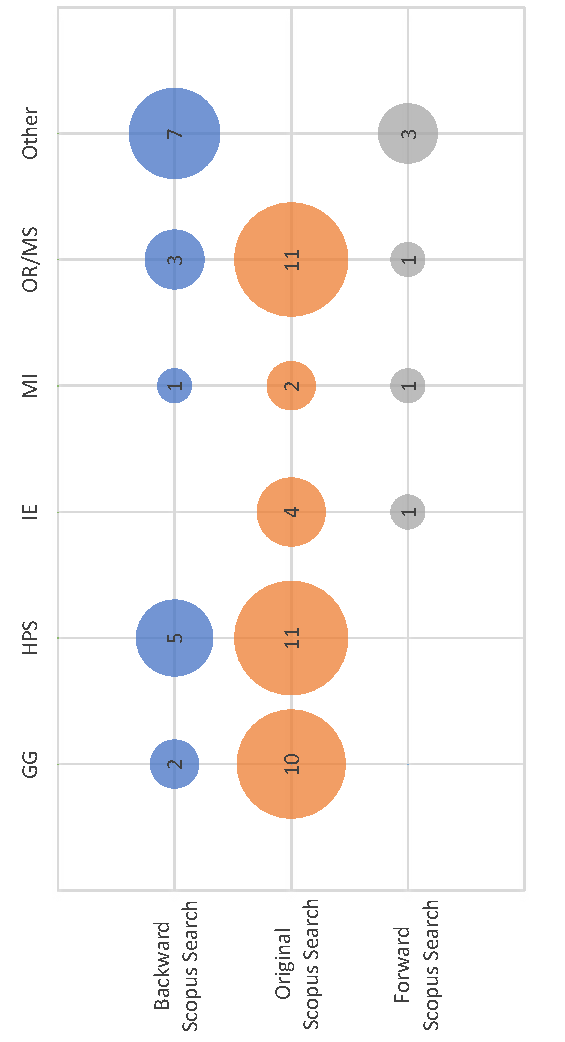
\includegraphics[scale = 0.6,angle=270]{Chapter2/Figures/Journal search chapter1.pdf}
  \caption{Number of publications broken down by journal categories}

\label{fig:journalsearch1}  
\end{figure}

Although there were only four and five papers within the MI and IE categories respectively, it is important to include these within \textcolor{black}{the} analysis as they \textcolor{black}{are under-represented areas and}
provide a different journal focus on patient pathways and \textcolor{black}{their} application.

To show the general trend of the research in this field, Figure \ref{fig:yearofpaper} displays the quantity of papers published every three years. Between 2000 and 2014, the number of papers published remained fairly stable with an upward trend from 2015. Within the last three years, 27\% of papers were published, highlighting that this area is becoming more widely researched. 

\begin{figure}[H]
\centering
  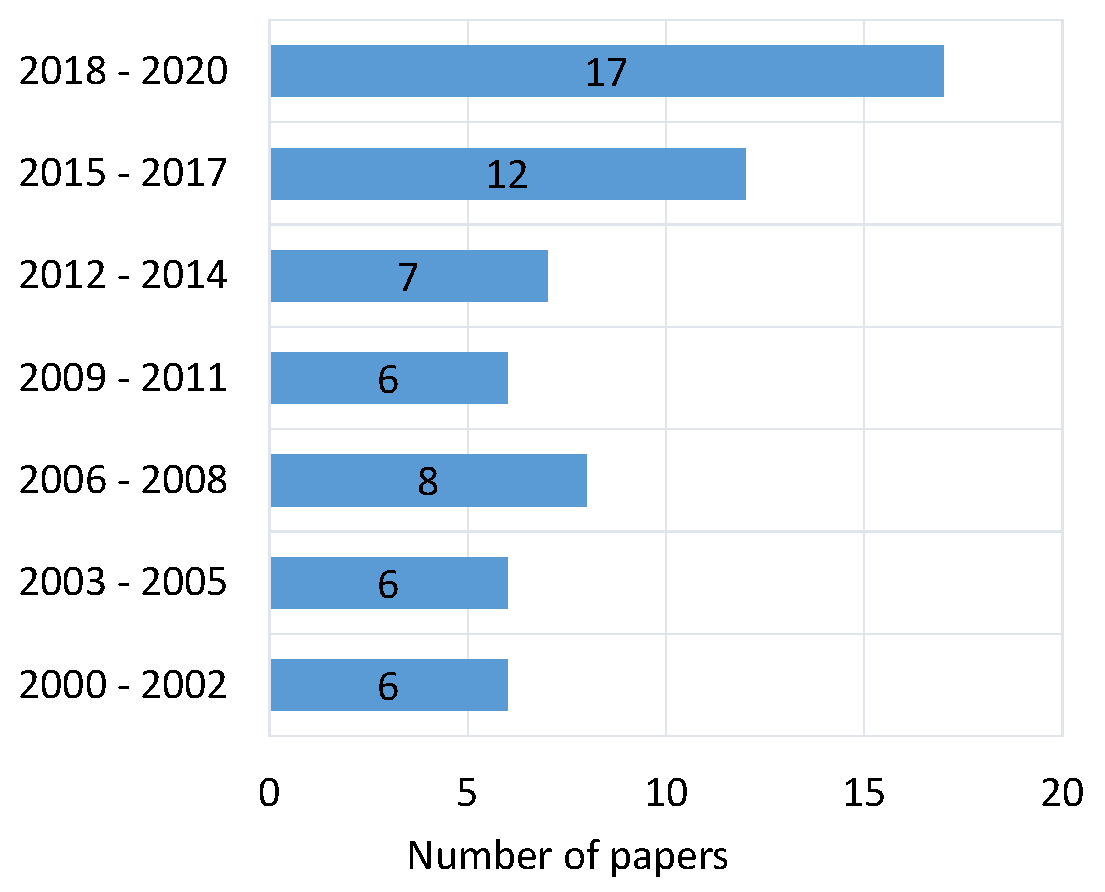
\includegraphics[scale=0.35]{Chapter2/Figures/Years2.pdf}
  \caption{Graph of publication year}
\label{fig:yearofpaper}    
\end{figure}

\subsubsection{Medical Context}
This subsection will analyse the medical context of the papers broken down into the medical setting and the condition area. The medical setting of a patient is the location where their care takes place, e.g., hospital ward or nursing home. The condition area focuses on the medical condition of the patient in the study and whether this was long-term such as dementia or acute, e.g., heart attack. Successful care planning should consider the entire pathway of a patient across multiple settings. It is often necessary to consider the next steps a patient will take to ensure appropriate resources and available capacity to avoid delays in discharge. It is also important to know the condition type of the patient as this will likely affect their discharge destination or the time required to stay within the care setting. 
\subsubsubsection{Medical Setting} \label{Medical Setting}
The medical setting of the paper was important to understand how care settings can work together for the planning of care for frail and elderly patients. The research focused on three main areas:

\begin{itemize}
    \item Single Hospital
    \item Multiple Hospitals
    \item Community Care
\end{itemize}

The community care grouping encompassed: Home care, long-term care, nursing care and hospice care, to meet the wide range of healthcare services that does not take place in a hospital setting.
Figure \ref{fig:VennDiag} shows a Venn diagram which breaks down the publications into the type of care settings. The numbers reveal there was a clear focus on both community care and single hospital settings.
.

\begin{figure}[h!]
\centering
  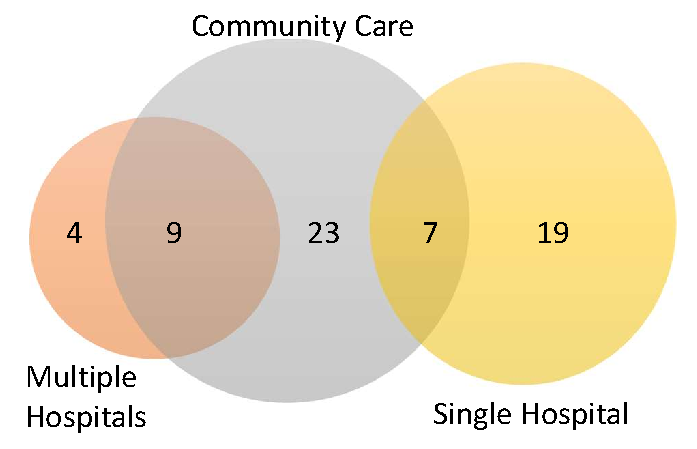
\includegraphics[scale=0.75]{Chapter2/Figures/Venn2.pdf}
\caption{Number of publications within each care setting}
\label{fig:VennDiag}  
\end{figure}


In total, there were 16 papers (26\%), which use care planning in a holistic manner. These papers were particularly interesting as they focused on the cross over between community care and either single or multiple hospitals. Papers \cite{Davari, Intrevado, Johnson, Lim,McClean,Patrick,Ragab, Walker, Zychlinski} focused on the intersection between community care and multiple hospitals whilst papers \cite{Faddy,Garg1,Garg2, Gordon1,Gordon2, Hare, Taylor} focused on single hospitals and community care.

A brief overview of Patrick \cite{Patrick} and Taylor et al. \cite{Taylor} is provided as these works are examples of community care with multiple hospitals and single hospital settings. 

Patrick \cite{Patrick} developed a Markov decision model that determined the required bed numbers in long-term care facilities in order to keep demand below a given threshold. Patrick also developed a simulation model to incorporate both hospital and community care demand to predict impact of policy implementations. These models have aided future capacity planning by comparing current practice against proposed alternative models.

The work conducted by Taylor et al. \cite{Taylor} involved modelling the time geriatric patients spent in hospital and in community care. The authors generated a stochastic compartmental Markov model with three hospital components: acute care; rehabilitative and long stay; two community components and an absorbing state. They were able to successfully provide short-term estimates and a better understanding of future bed usage within geriatric hospital settings.

\subsubsubsection{Illness/Disease Focused Papers}
There were eight papers which focused on a specific illness/disease often suffered by the frail and elderly. These illnesses were as follows: dementia \cite{Cepoiu}, falls \cite{Franklin}, gastrointestinal \cite{Abe}, heart failure \cite{Azad, Kul, Shaw} and hip fractures \cite{Beaupre, Wallace}. Seven of the eight papers focused on a single hospital setting and \textcolor{black}{the remaining paper} focused on community care \cite{Cepoiu}. \textcolor{black}{There were a further} eight papers which focused on an inpatient \textcolor{black}{department}\textcolor{black}{:} an emergency department \cite{Patrick, Rashwan, Rossille,Trevisan} or a geriatric ward \cite{Christodoulou, Franck, Gorunescu,Marshall3}. Interestingly, none of these \textcolor{black}{16} papers used care planning across multiple settings. \textcolor{black}{The recovery times for frail and elderly patients is usually longer than the general population. Often, they will require further care within the community once they are ready to be discharged. If there is insufficient resources or lack of availability within the community, then these patients may have to remain in hospital, causing bed blocking.}


\subsubsubsection{Community Care Focused Papers}
\textcolor{black}{There were} 23 papers which had community care as the \textcolor{black}{only} setting.  \textcolor{black}{Six of these papers concentrated} on the overlap and movement between settings in community \cite{Bae, Gassoumis, YLi,Bidhandi,Welberry, Zhang1}. Lin et al. \cite{Lin} focused on day care whilst \cite{Eveborn, Grenouilleau, Guo, Yalcindag} \textcolor{black}{studied} home care. The remaining papers focused on either nursing care \cite{Arling,Borowiak, Muramatsu} \textcolor{black}{or} long-term/aged related care facilities \cite{Ambagtsheer, Arvelo, Cepoiu, Desai, Eggink, Katsaliaki, Kerpershoek, Tao, Xie}. This shows that within the grouping of community care there \textcolor{black}{were} a wide range of different settings being \textcolor{black}{analysed}.


For \textcolor{black}{frail and elderly} care mapping to be successful, the journey of a patient should be documented, which will depend on the type of illness they are suffering \textcolor{black}{from. Therefore it} is important for more research to be conducted into specific illnesses \textcolor{black}{and healthcare} settings. \textcolor{black}{M}onitoring the journey of a patient from admittance through to discharge\textcolor{black}{, may become a valuable tool in order} to predict long\textcolor{black}{-}term demands and capacity planning.

\subsubsubsection{Condition Area}
A classification which has been commonly used within healthcare literature reviews is the condition area of the patient \cite{Aspland,YZhang}. These \textcolor{black}{condition areas} are often categorised \textcolor{black}{as either:} acute \textcolor{black}{or} chronic.

\begin{itemize}
    \item Acute - Medical conditions that are brought on unexpectedly\textcolor{black}{, e.g.}, heart failure, or patients undergoing or recovering from a surgical procedure\textcolor{black}{, e.g.}, femur fracture.
    \item Chronic - Medical conditions that are prolonged and rarely cured, \textcolor{black}{e.g.}, dementia.
\end{itemize}

Often chronic conditions can develop and cause an acute condition, \textcolor{black}{and likewise}, if untreated an acute condition can often become chronic. It is therefore important for research to be focused within both strands of conditions, especially when considering \textcolor{black}{frail and elderly} patients. These patients often have many chronic conditions which require long-term care, however they can easily become more serious conditions requiring immediate care.

Figure \ref{fig:Condition} displays the quantity of papers in each condition category.

\begin{figure}[h!]
\centering
  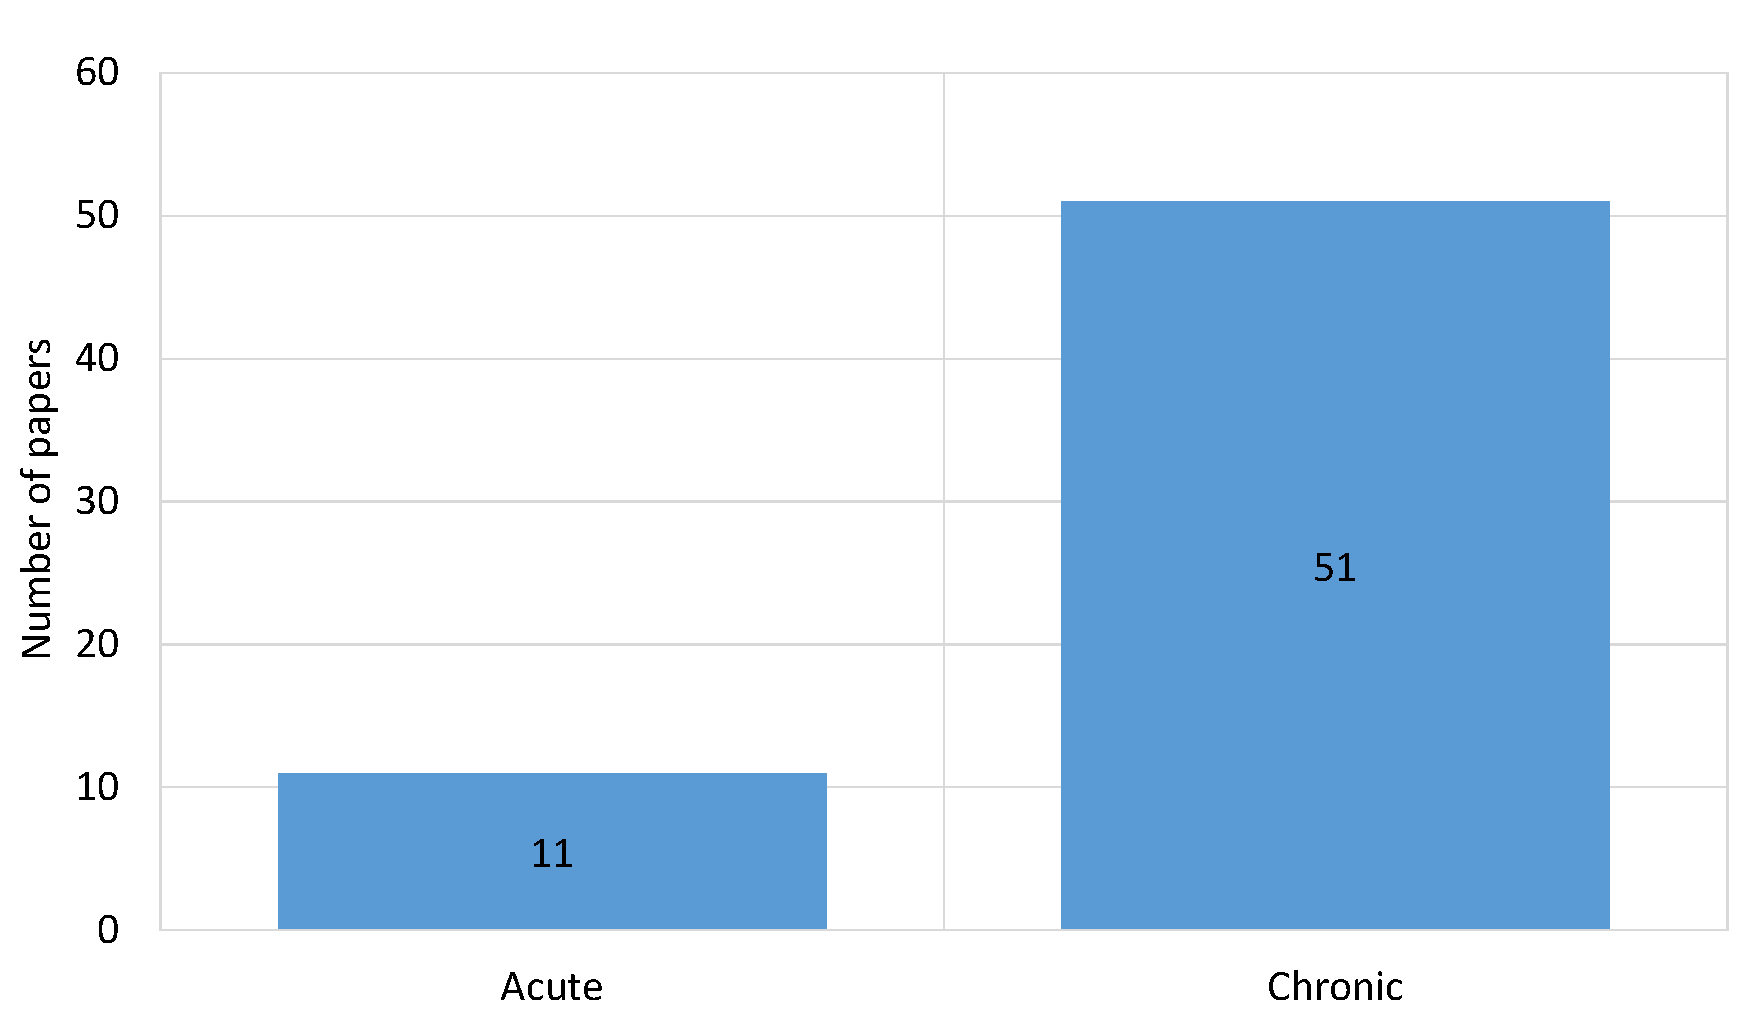
\includegraphics[scale=0.3]{Chapter2/Figures/AcuteChronic.pdf} 
  \caption{Condition categories of publications}
  \label{fig:Condition}
\end{figure} 

Within the elderly population, there are many people who have multiple long\textcolor{black}{-}term conditions (MLTC), which may explain why there \textcolor{black}{were} many papers that focus on chronic conditions. \textcolor{black}{Eleven} papers focused on the acute care setting \cite{Abe, Azad, Franklin, Kul, Onggo, Rashwan, Rossille, Shaw, Silvester, Trevisan, Wallace}. %However, it would be expected for there to be more than eleven papers that focused on the acute care setting \cite{Abe, Azad, Franklin, Kul, Onggo, Rashwan, Rossille, Shaw, Silvester, Trevisan, Wallace}.
\textcolor{black}{This is surprising given }% may be assumed as
frail and elderly patients are more likely to suffer from acute conditions as a result from chronic illness.
% Many \textcolor{black}{frail and elderly} patients would be waiting for surgical treatment, such as cataract surgery or knee/hip replacements but cannot access these services because of long waiting lists.
The eleven papers were all based in the single hospital setting with no overlap between community care \textcolor{black}{(}Figure \ref{fig:HospCondition}\textcolor{black}{)}.

\begin{figure}[H]
\centering
  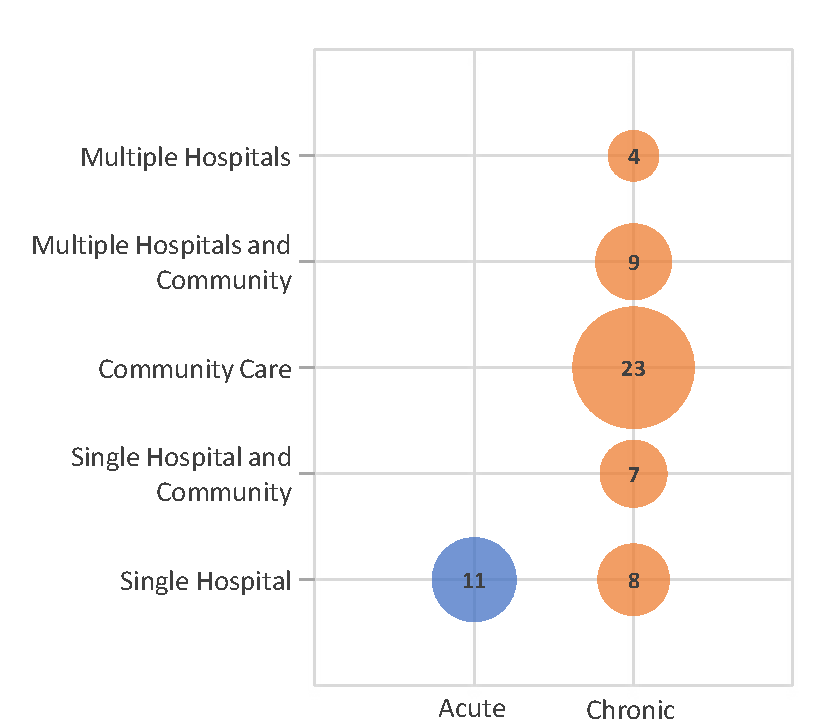
\includegraphics[scale =0.6]{Chapter2/Figures/HospitalCondition1.pdf}
\caption{Cross analysis of setting and condition categories of publications}
\label{fig:HospCondition}  
\end{figure} 



\subsubsection{Methodological Content}
This subsection will analyse the technical side of the research. Firstly\textcolor{black}{,} discussing the research aims, \textcolor{black}{then} moving on to the planning decision levels discussed in Hulshof et al.'s taxonomy \cite{PHulshof}. Finally, the different OR/MS methods used within \textcolor{black}{frail and elderly} care planning are identified.

\subsubsubsection{Research Aims}
The literature can be grouped into three main aims of the papers in terms of care planning: \textcolor{black}{e}xamining, forecasting and improving. These categories indicate the direction of the research and the main interest to the authors. 

\begin{itemize}
    \item Examining - Using OR methods to determine how a care plan was performing\textcolor{black}{, e.g.}, characteristics of patients who move within community care \cite{Gassoumis}, hospital outcomes following an updated care pathway \cite{Wallace}.
    \item Forecasting - Predicting future scenarios with the current care plan in place\textcolor{black}{, e.g.}, forecasting length of stay in hospital and community care \cite{Gordon2}, capacity planning in community care settings \cite{Bidhandi}.
    \item Improving - Improvements were made or suggested to \textcolor{black}{enhance} the quality of care planning\textcolor{black}{, e.g.}, improve elderly care in hospital \cite{Ragab}, improving quality and efficiency in home care \cite{Eveborn}.
\end{itemize}

Figure \ref{fig:Aims} displays the quantity of papers in each \textcolor{black}{research} aim category.

\begin{figure}[H]
\centering
    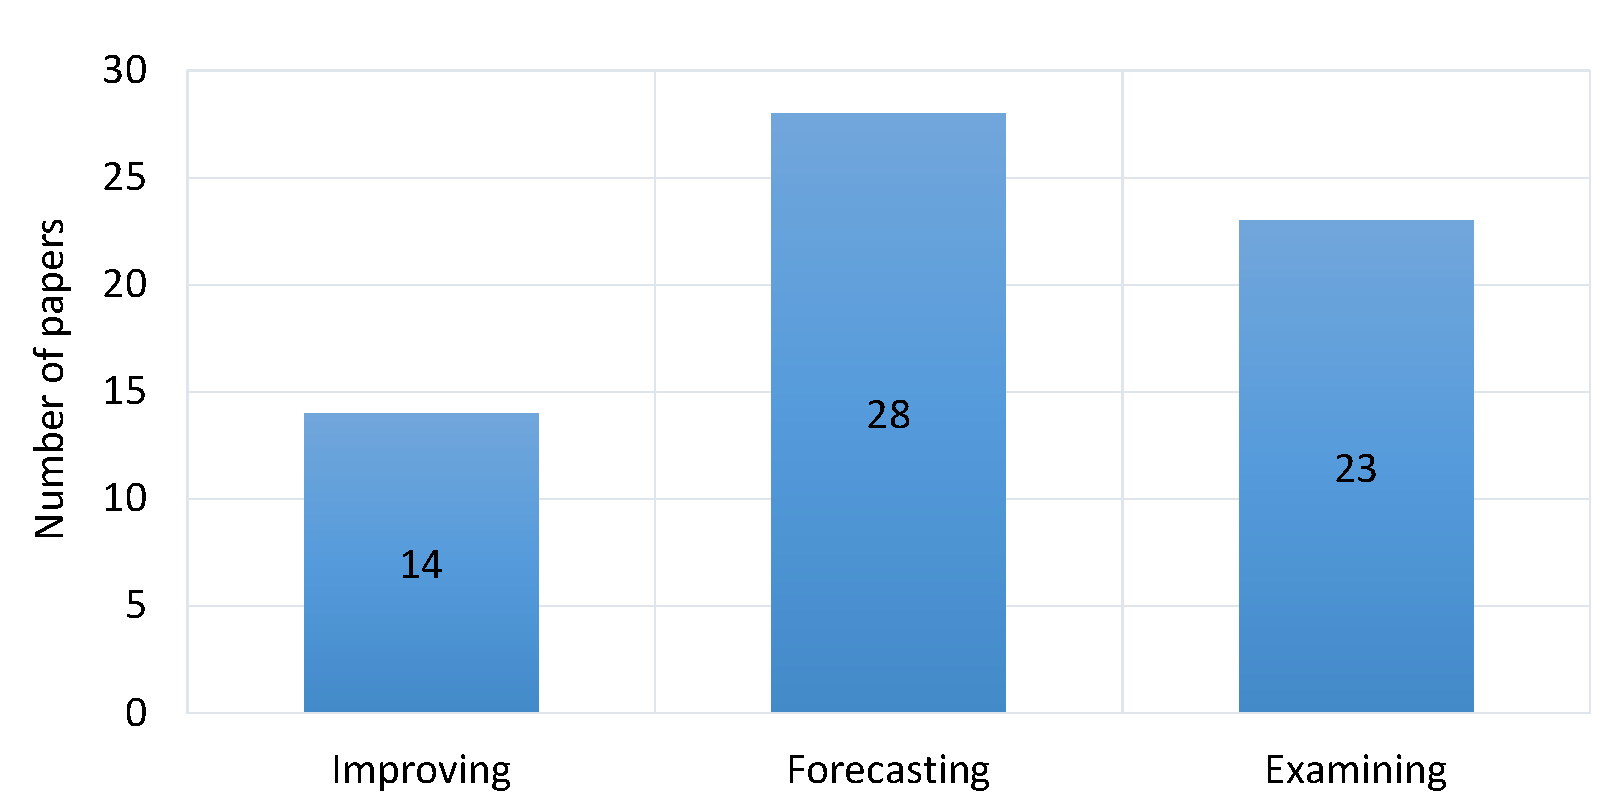
\includegraphics[scale = 0.3]{Chapter2/Figures/Focus1.pdf}
   \caption{Research aims of the papers}
   \label{fig:Aims}
\end{figure}

\textcolor{black}{There were three papers which considered a multiple combination of the research aims.} Abe et al. \cite{Abe} examined how polypharmacy \textcolor{black}{affected} gastrointestinal surgery patients, whilst also identifying the effects on length of stay if measures \textcolor{black}{reducing} polypharmacy were implemented. Garg et al. \cite{Garg2} and Patrick \cite{Patrick} both have improving and forecasting aims: Garg et al. focused on improving admission scheduling with resource forecasting and Patrick focused on improving waiting times along with capacity planning. All three of these papers, focused on a single hospital setting.

The results show most papers aim to forecast \textcolor{black}{frail and elderly} patients in the system. Out of the 28 papers, 16 focused on predicting future demands and how \textcolor{black}{the corresponding} department\textcolor{black}{s} would be required to adapt to this change \cite{Ambagtsheer, Bae, Borowiak, Christodoulou,  Davari, Desai, Gorunescu, Grenouilleau, Hare, Johnson, Katsaliaki, YLi, Bidhandi, Patrick,Zhang1, Zhang2}. A further nine papers aimed to predict the length of stay of patients in \textcolor{black}{hospitals or within community care} \cite{Abe, Gordon2, Heggestad, Marshall1, Marshall2, Marshall3, Shaw, Taylor, Xie}. Surprisingly, of these nine, one author was co-author on five of these papers, suggesting that the research within this field is limited to a few research \textcolor{black}{teams} \cite{Gordon2, Marshall1, Marshall2, Marshall3, Shaw}.

Fourteen papers focused on making improvements to an aspect of the pathway. Five of these aimed to improve the flow of patients \cite{Chaussalet, Hamdani, Rashwan, Silvester, Trevisan}. Only three papers had the primary focus on improving patient care \cite{Eveborn, Ragab, Rossille}. Their results highlighted the importance of appropriate care to the elderly, which in Rossille et al.'s \cite{Rossille} paper can be achieved by successfully scheduling patients in an emergency department and not categorising these patients by their symptoms. Ragab et al. \cite{Ragab} used simulation modelling to improve the management of frail patients \textcolor{black}{by introducing intermediate care beds for those} admitted to acute hospitals. Eveborn et al. \cite{Eveborn} used the vehicle routing problem to improve quality \textcolor{black}{for} patients receiving home care.

\subsubsubsection{Planning Decisions}
Hulshof et al's. \cite{PHulshof} research on taxonomic classification in healthcare systems highlighted a hierarchy of decision making techniques. There \textcolor{black}{were} three different decision levels discussed: \textcolor{black}{s}trategic, tactical and operational. A brief description is given as follows:

\begin{itemize}
    \item Strategic planning focuses on structural decision making such as determining the locations of facilities or resource capacities\textcolor{black}{, these} often have a long planning time.
    \item Tactical planning addresses the execution of strategic plans on the mid-horizon planning time, \textcolor{black}{e.g.}, staffing levels.
    \item Operational planning analyses short-term decisions and focuses on the individual patient and resources. \textcolor{black}{Patient appointment scheduling} would be an example of this.
\end{itemize}

Figure \ref{fig:PlanningDecision} displays the breakdown of publications by planning decision level.

\begin{figure}[H]
\centering
    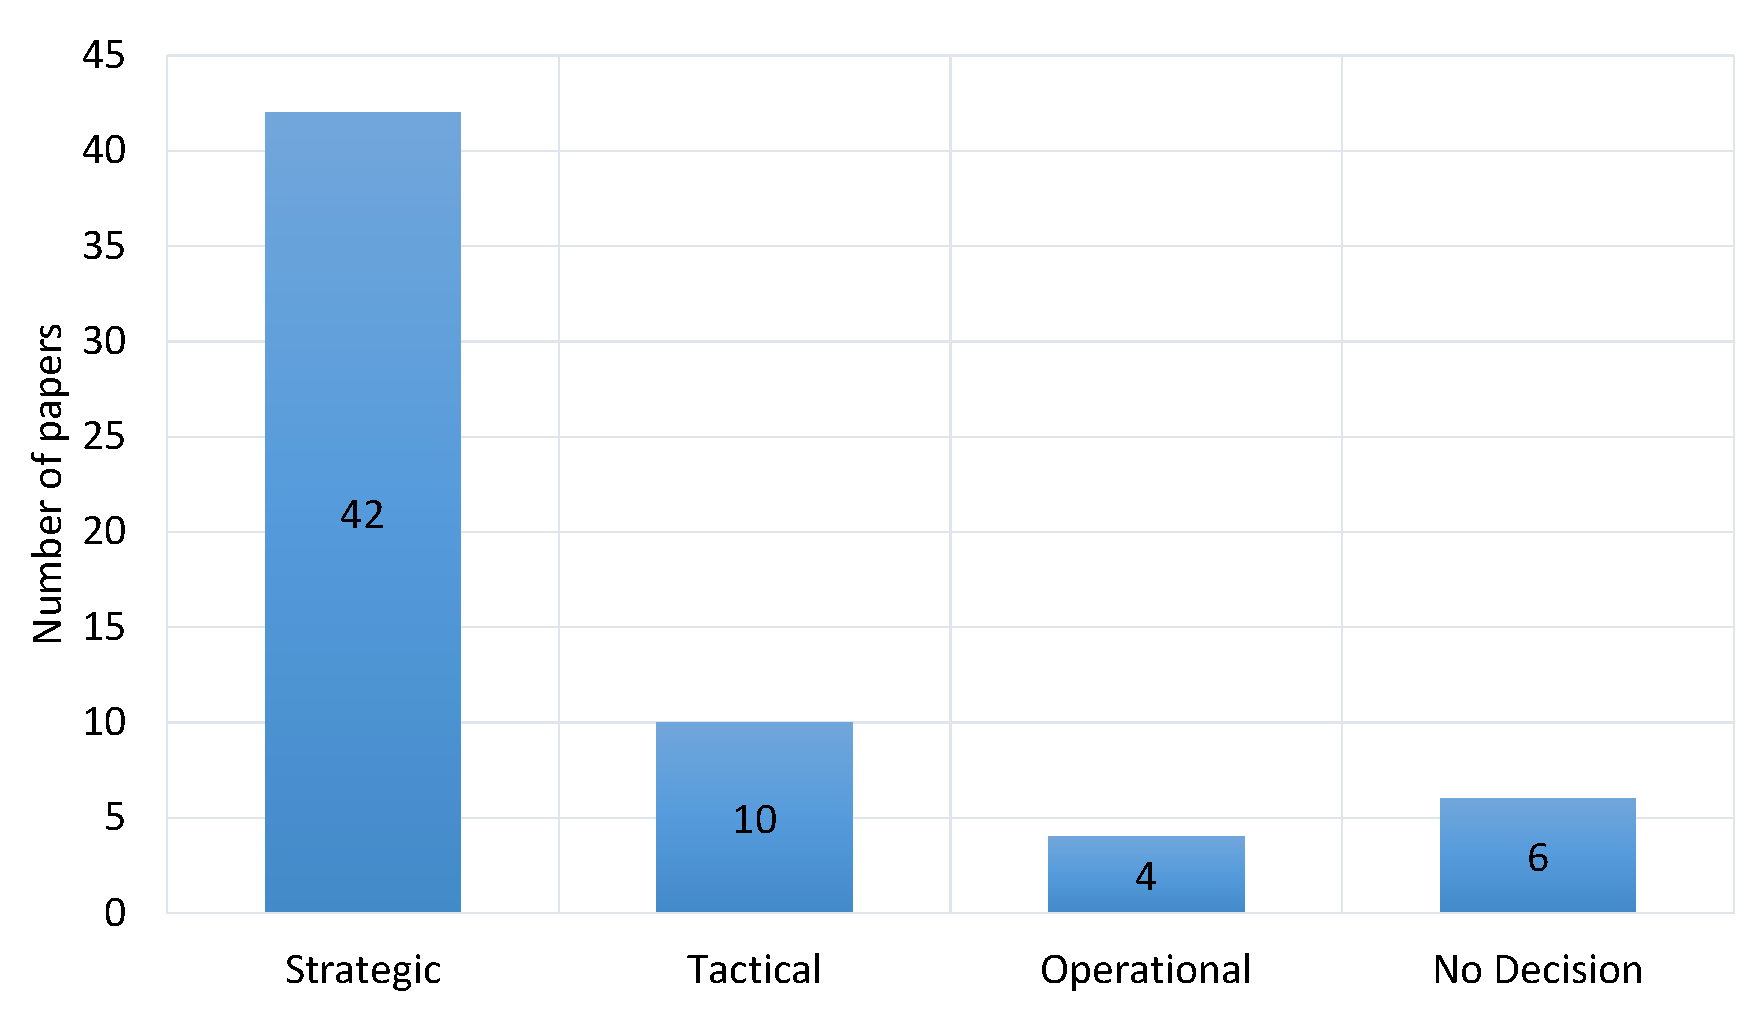
\includegraphics[scale = 0.3]{Chapter2/Figures/Planning1.pdf}
   \caption{Planning decision level of publications} \label{fig:PlanningDecision}
\end{figure}

The majority of papers focused on strategic planning, with a high concentration on capacity planning and placement policy. Xie et al. \cite{Xie} used strategic planning and created a Markov model to \textcolor{black}{represent} the length of stay of the elderly moving within and between residential and nursing homes. By developing this model, it aimed to assist planning authorities to fully understand the pattern of resource usage within their local area. Further work included \textcolor{black}{an} extension of their model to incorporate \textcolor{black}{particular} attributes of patients, \textcolor{black}{e.g.,} age, gender and physical conditions, to predict difference\textcolor{black}{s} in survival by \textcolor{black}{treatment locations}.

The number of papers \textcolor{black}{(two)} on the operational planning level is smaller than \textcolor{black}{the} number of papers \textcolor{black}{(six)} that have no \textcolor{black}{planning} decision \textcolor{black}{level}. The results show\textcolor{black}{ed} that care planning for \textcolor{black}{frail and elderly} pathways \textcolor{black}{was} being addressed on some scale across all three decision levels\textcolor{black}{;} day\textcolor{black}{-}to\textcolor{black}{-}day\textcolor{black}{; mid-level planning;} long-term, wider policy decisions. However, as there were substantially \textcolor{black}{fewer} papers in the tactical and operational decision levels it would suggest these areas are more difficult to plan in \textcolor{black}{frail and elderly} healthcare.

Two of the four operational planning papers focused on staff scheduling \cite{Eveborn,Grenouilleau} and the other two focused on readmission of patients \cite{Gordon1} and treatment outcomes \cite{Kul}. Kul et al. \cite{Kul} evaluated the effect \textcolor{black}{of the} heart failure care pathway \textcolor{black}{on} geriatric patients. Logistic regression showed \textcolor{black}{positive results supporting the use of} care pathways\textcolor{black}{,} highlighting reduced mortality and readmission rates along with \textcolor{black}{no} increase in hospital costs.

Figure \ref{fig:PlanningSetting} displays the cross analysis between the planning decision and the \textcolor{black}{medical} setting. \textcolor{black}{To} some \textcolor{black}{degree}, tactical planning levels \textcolor{black}{were} addressed in each setting, although the operational papers \textcolor{black}{had} only been addressed within community care and single hospital settings. 

\begin{figure}[H]
\centering
        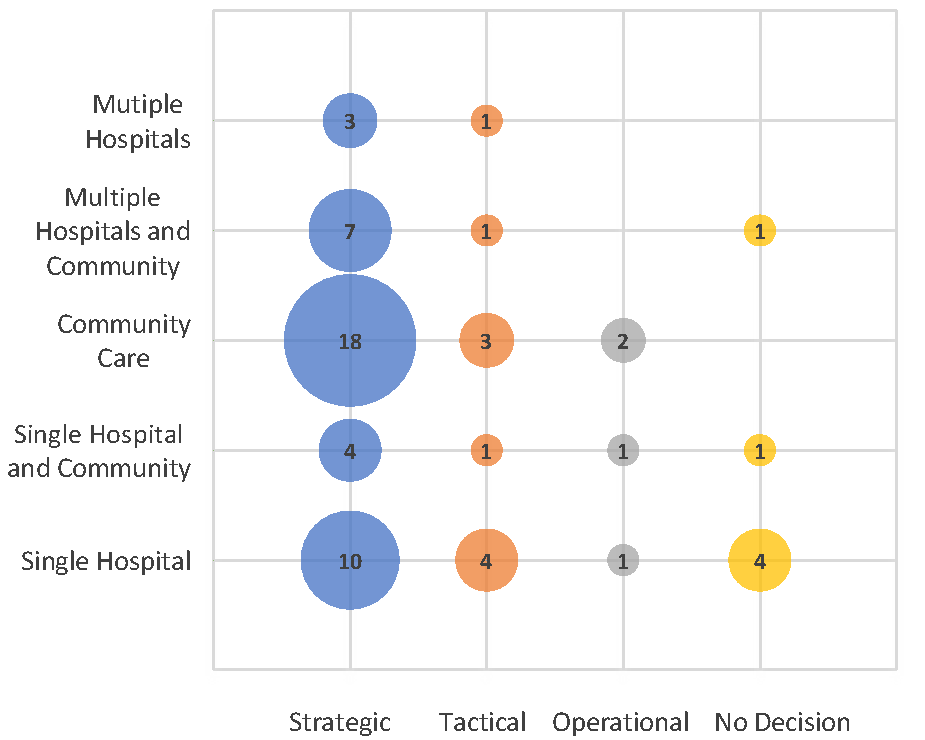
\includegraphics[scale = 0.6]{Chapter2/Figures/PlanningSetting1.pdf}
        \caption{Cross analysis of planning decision and setting}
    \label{fig:PlanningSetting}
\end{figure}

Hulshof et al. \cite{PHulshof} analysed the taxonomy for papers within the OR/MS JCR category. This has been further extended to include four additional JCR categories. The cross analysis can be seen within Figure \ref{fig:PlanningJCR}.

\begin{figure}[H]
\centering
 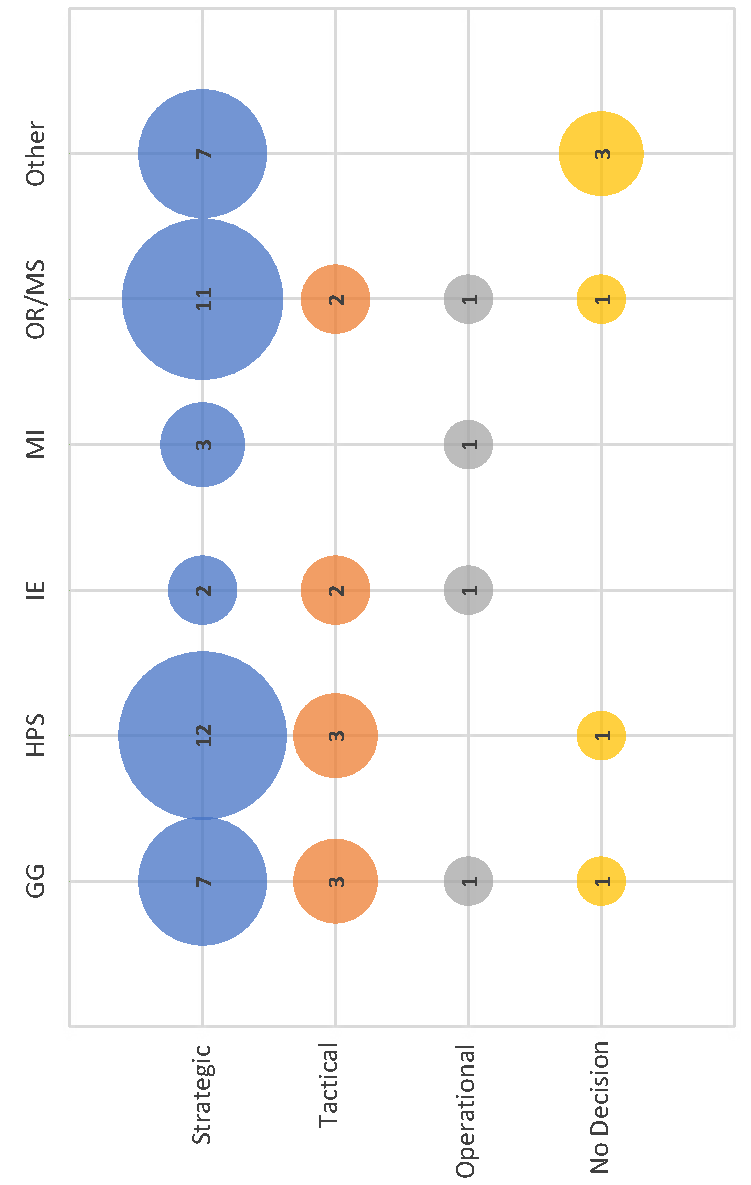
\includegraphics[scale = 0.5,angle=270]{Chapter2/Figures/JCRDecision1.pdf}
 \caption{Cross analysis of JCR category and decision level}
   
    \label{fig:PlanningJCR}
\end{figure}

Figure \ref{fig:PlanningJCR} shows there is a spread of decision levels against each JCR category. It demonstrate\textcolor{black}{s} that the decision level taxonomy discussed within Hulshof et al. \cite{PHulshof} \textcolor{black}{can} be successfully applied to JCR categories other than OR/MS. 

\subsubsubsection{OR/MS Methods}
The final area for analysis was investigating the OR/MS methods that have been utilised within these studies. There has been a variety of different OR/MS techniques which have been used to demonstrate the effectiveness of care planning designs specifically for the \textcolor{black}{frail and elderly}. Figure \ref{fig:Mathematical} demonstrates the quantity of each of these methods, with statistical analysis encompassing a wide range of traditional \textcolor{black}{statistical}/operational analysis techniques, including Cox's regression analysis \cite{Heggestad}, mixed exponential distributions \cite{Harrison} and time survival analysis \cite{Muramatsu}. Optimisation \textcolor{black}{included} %linear programming,
mixed integer programming \textcolor{black}{\cite{Davari}} and quadratic programming \textcolor{black}{\cite{Tao}}. \textcolor{black}{Simulation} \textcolor{black}{included} %agent based simulation,
discrete event simulation \textcolor{black}{\cite{Zhang1}} 
%, Monte Carlo simulation
and system dynamics \textcolor{black}{\cite{Cepoiu}}.
There were two papers which focused on multiple methods.

\begin{figure}[H]
\centering
    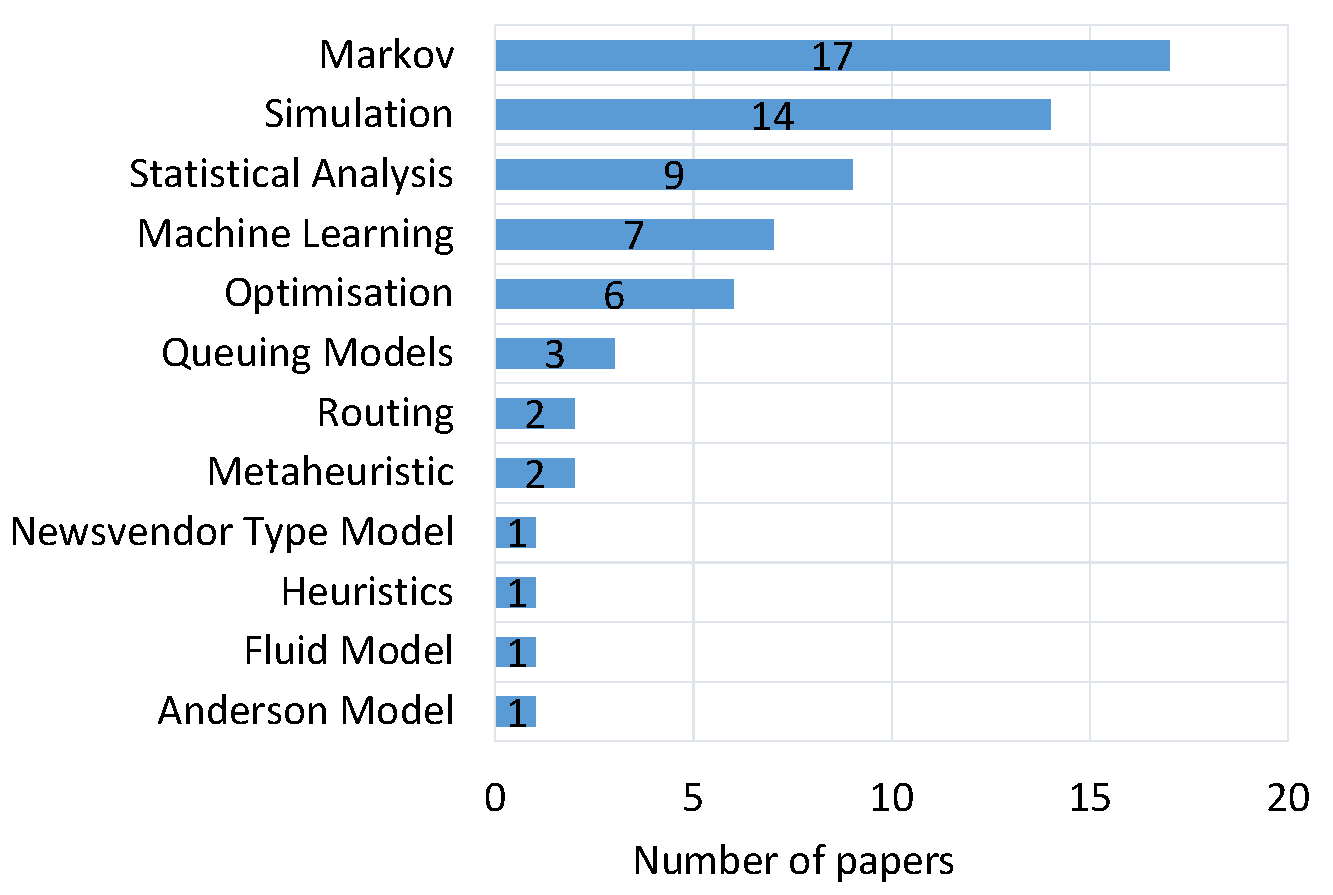
\includegraphics[scale = 0.45]{Chapter2/Figures/ModelsGraph.pdf}
    \caption{Quantity of publications by mathematical method}
    \label{fig:Mathematical}
\end{figure}

Patrick \cite{Patrick} as discussed in \textcolor{black}{Section} \ref{Medical Setting} used discrete event simulation along with a Markov decision process model to predict demand for long-term care. 

Mohammadi Bidhandi et al. \cite{Bidhandi} used both simulation and queueing theory methods to plan demand capacities within community care. They focused on six services and ran their optimised queueing model through a simulation to determine transient behaviours of the system. By combining these two methods, capacities \textcolor{black}{were} optimised over the entire network at one time, instead of considering them as separate isolated units.

Table \ref{tab:MethodHosp} shows the breakdown of each OR/MS method and its corresponding setting. The seven papers which looked at the overlap between single hospitals and community care all used Markov methods. This may suggest that Markov methods are the most applicable ones to this setting, particularly for frail and elderly individuals. The data available may also lend itself well to fit into a Markov model. Expanding upon this, when analysing both single and multiple hospitals with community care, only Markov, simulation and statistical analysis methods \textcolor{black}{were} used, suggesting these methods \textcolor{black}{were} useful when applied to multiple services at the same time. This leaves room \textcolor{black}{in these settings,} for further \textcolor{black}{research} \textcolor{black}{using alternative} OR/MS methods to \textcolor{black}{the Markov model.} 

Community care settings used the widest range of methods, thirteen in total, for care planning. This showed the data available within community care can accommodate a variety of methods. \textcolor{black}{T}here is potential for further investigation and expansion into the methods utilised as an area for future research.


\begin{landscape}
\begin{table*}[h!]
\centering
\scalebox{0.7}{%
    \begin{tabular}{@{}cccccc|c@{}} \toprule
 &
\textbf{Single Hospital} & \textbf{Single Hospital and Community} & \textbf{Community Care} & \textbf{Multiple Hospitals and Community} & \textbf{Multiple Hospitals} &\textbf{Total} \\ \midrule
%\textbf{Markov}  & 6 & 7 & 1 & 2 & 1 & 17 \\
\textbf{Markov} & \cite{Christodoulou, Franklin, Hamdani, Marshall1,Marshall2,Shaw} & \cite{Faddy, Garg1, Garg2, Gordon1, Gordon2, Hare, Taylor} & \cite{Xie} & \cite{McClean, Patrick} & \cite{Marshall3} & 17\\
\textbf{Simulation} &\cite{Onggo,Rashwan,Zhang2}&&\cite{Bae, Cepoiu,Desai,Eggink,Katsaliaki,Bidhandi, Zhang1}&\cite{Patrick, Ragab,Walker}&\cite{Franck}& 14\\
\textbf{Statistical Analysis} &\cite{Azad,Beaupre,Silvester,Wallace}&&\cite{Borowiak,Guo,Muramatsu}&&\cite{Harrison,Heggestad}& 9\\
\textbf{Machine Learning} &\cite{Abe,Kul, Rossille, Trevisan}&&\cite{Ambagtsheer,Gassoumis,Welberry}&&& 7 \\
\textbf{Optimisation} & &&\cite{Arling,Arvelo,Tao}&\cite{Davari, Intrevado, Johnson}&&6\\
\textbf{Queueing models} &\cite{Chaussalet,Gorunescu}&&\cite{Bidhandi}&&&3 \\

\textbf{Metaheuristic}&&&\cite{Grenouilleau,Lin}&& &2 \\
\textbf{Routing}&&&\cite{Yalcindag}&\cite{Lim}& &2 \\
\textbf{Anderson Model}&&&\cite{Kerpershoek}&& &1 \\
\textbf{Fluid model}&&&&\cite{Zychlinski}&& 1 \\
\textbf{Heuristics}&&&\cite{Eveborn}&& &1 \\
\textbf{Newsvendor type model}&&&\cite{YLi}&&& 1 \\

\midrule
\textbf{Total} & 19 & 7 & 24 & 10 & 4 & 64\\
\bottomrule
\end{tabular}
}\caption{Setting and OR/MS method used within the published research}

\label{tab:MethodHosp}
\\
[8pt]
\caption*{Note: Mohammadi Bidhandi et al. \cite{Bidhandi} and Patrick \cite{Patrick} utilise two methods and therefore appear twice in the table. This results in a total of 64.}
\end{table*}

\end{landscape}

Figure \ref{fig:Mathematical} and Table \ref{tab:MethodHosp} highlight that Markov models \textcolor{black}{were} the most frequent method used, followed by simulation and statistical analysis. Within these 17 papers, there were a variety of Markovian methods utilised, however these \textcolor{black}{were} subgrouped into continuous and discrete time models. Figure \ref{Fig:markov} shows the breakdown of the Markov category from Figure \ref{fig:Mathematical}. Continuous time Markov models \textcolor{black}{were} more often used with a total of fourteen papers \cite{Christodoulou,Faddy,Franklin, Garg1, Gordon1, Gordon2, Hamdani, Marshall1, Marshall2, Marshall3,McClean, Shaw, Taylor, Xie}. There were a variety of different types of continuous time models with many focusing on Coxian phase-type Markov models. There were three papers which used discrete time \cite{Garg2,Hare, Patrick} to model \textcolor{black}{frail and elderly} patients.

\begin{figure}[H]
\centering
    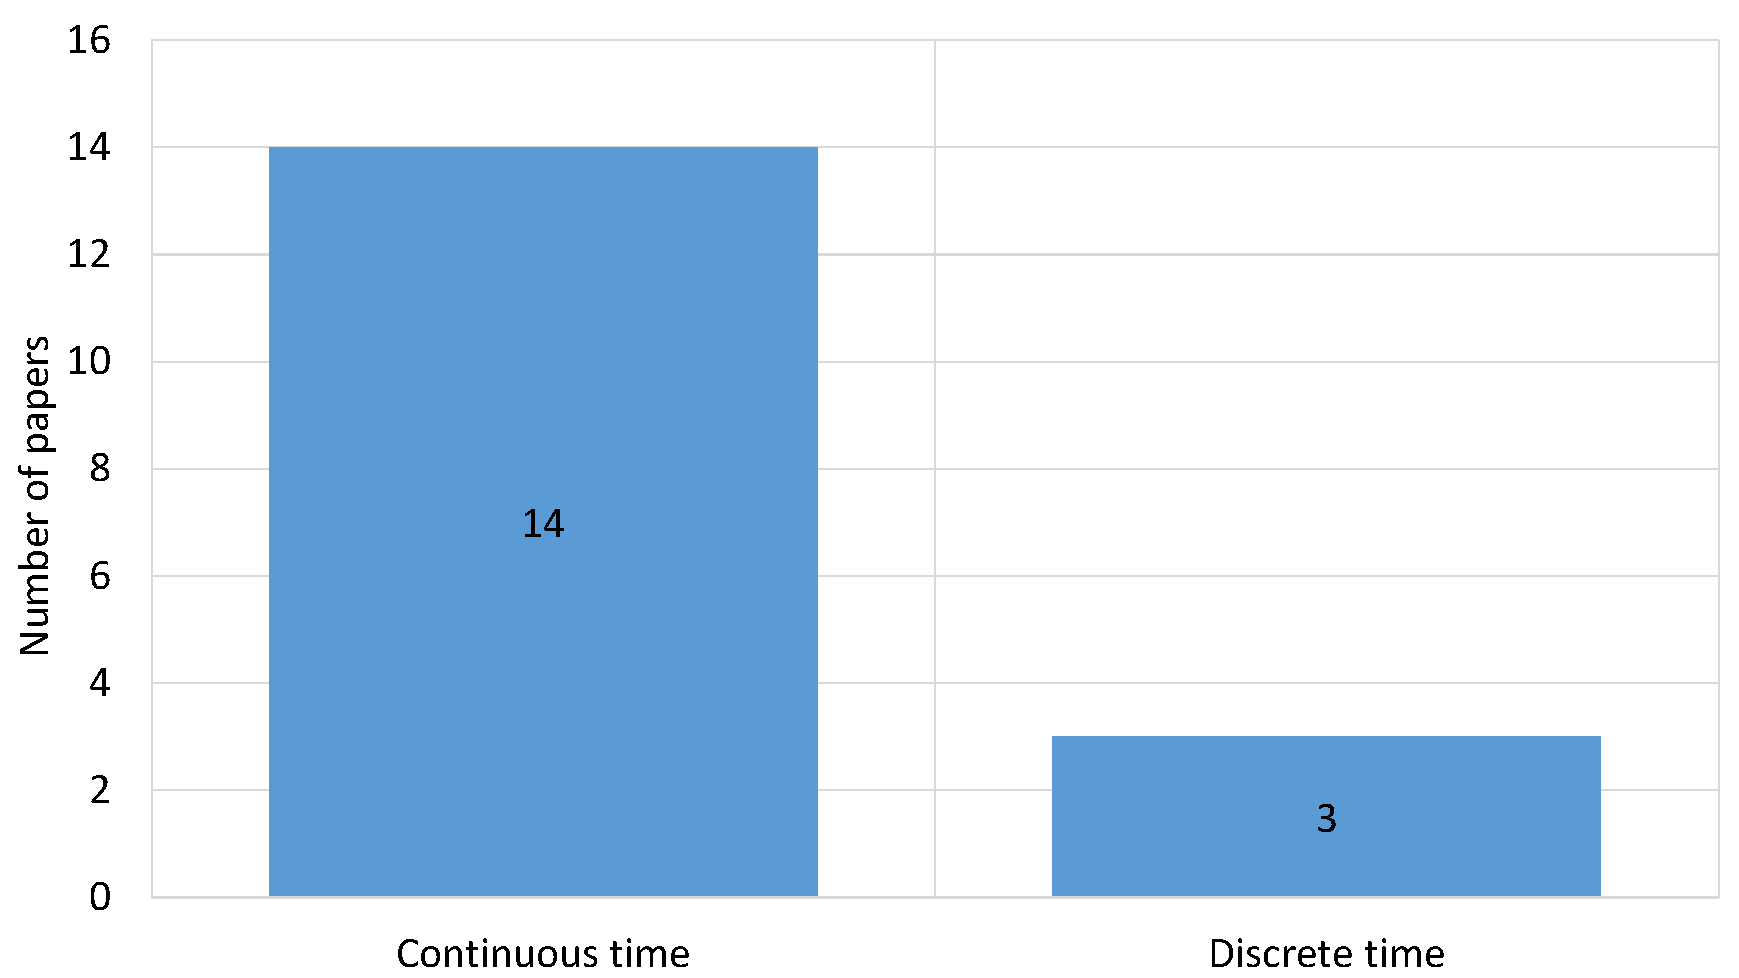
\includegraphics[scale = 0.3]{Chapter2/Figures/Markov1.pdf}
 \caption{Further breakdown of the Markov model category}
 \label{Fig:markov}
\end{figure}

\subsubsection{Common Themes}
\textcolor{black}{Section \ref{sec:Classification}} has provided an overview of the work on care planning \textcolor{black}{for} frail and elderly. Markov models \textcolor{black}{were} \textcolor{black}{the most common method} applied to healthcare settings. In more recent years, \textcolor{black}{there has been the }emergence of newer techniques being applied to \textcolor{black}{healthcare,} i.e., metaheuristics, the Anderson Model and fluid models. Strategic planning remained the most common planning decision level across the OR/MS methods, showing \textcolor{black}{research was} being accomplished in longer term care planning. There has been a wider spread of research aims across the papers, \textcolor{black}{although}, the majority tend to focus on forecasting future scenarios rather than improving the current systems in place. Finally\textcolor{black}{,} the emphasis of these papers \textcolor{black}{has} been on single settings, whether this be within a hospital or the community. The current research provides a wide range of different techniques \textcolor{black}{for readers to apply to their own hospital or community care facility. However,} there \textcolor{black}{remains scope} for \textcolor{black}{future} research to be conducted in \textcolor{black}{the frail and elderly patient setting.}

\subsection{Research Gaps} \label{Sec:Research} 
The literature found within this review cover\textcolor{black}{ed} a wide range of facilities, locations and patient types within frail and elderly care planning. Despite this variety, the majority of papers fit into a few groupings as discussed previously, with heavy focus on certain methods and locations.

\subsubsection{Gaps in terms of Methodology}
Across 62 papers, there were twelve different methods utilised, with a heavy focus on Markov and simulation. Research conducted between 1990 and 2015 has shown that the most common OR methods used in hospital applications were discrete event simulation and deterministic modelling (optimisation) \cite{Abe1,Abe2}. It \textcolor{black}{was} interesting to see the disparities between methods within \textcolor{black}{frail and elderly} care and general hospital applications. In the simulation method category \textcolor{black}{(}Table \ref{tab:MethodHosp}\textcolor{black}{)}, only five papers used discrete event as their simulation method \cite{Franck, Katsaliaki, Onggo, Zhang1, Zhang2} and papers focusing on optimisation techniques were embedded within other methods \cite{Bae, Garg1, Lin,Bidhandi, Silvester, Tao, Yalcindag, Zhang2}. 

 Within Abe et al.’s paper \cite{Abe2}, the statement was made that the introduction of the Patient Protection and Affordable Care Act in 2010 (USA), has led to hospitals \textcolor{black}{being required} to improve quality of care \textcolor{black}{and} alongside this, there has also been an increase in the demand of services in \textcolor{black}{U.S.} hospitals. \textcolor{black}{The} seven papers \textcolor{black}{that were based on data from the \textcolor{black}{U.S.} post 2010, focused} on capacity planning and improving outcomes \cite{Arling,Bae, Gassoumis,Guo,YLi, Wallace, Zychlinski}. This suggests that the implementation of Government policy provides another avenue for research topics and should be closely monitored when identifying new areas to \textcolor{black}{study}.
 
 Although healthcare data may lend itself well to some OR/MS methods explaining their higher frequency of papers (Markov, simulation, statistical analysis and machine learning), the remaining eight methods highlight the potential for further exploration into \textcolor{black}{these fewer applied} techniques. Soft OR methods, even though included in the search criteria, did not result in any papers being identified. This leaves potential for \textcolor{black}{research} using these techniques, such as soft systems methodology, and applying this to \textcolor{black}{frail and elderly} healthcare.
 
\subsubsection{Gaps on the Intersection between Research Aims and Decision Levels}
Successful care planning should consider long-term and day\textcolor{black}{-}to\textcolor{black}{-}day planning. The work has highlighted a large number of papers with strategic decision levels (long-term), with only fourteen papers analysing tactical and operational approaches, ten and four \textcolor{black}{combined. Reviewing} the 23 community care papers, three focused on tactical planning \cite{Borowiak, Eggink, Yalcindag}, and two with operational planning \cite{Eveborn, Grenouilleau}. Despite being long-term care facilities, day\textcolor{black}{-}to\textcolor{black}{-}day planning of staff, resources and occupancy demands should be investigated for improving care planning. Such investigation could provide an interesting avenue to explore further, \textcolor{black}{by} comparing how factors vary day\textcolor{black}{-}to\textcolor{black}{-}day for private care companies compared to \textcolor{black}{government} funded elderly care services. Operational planning levels were \textcolor{black}{addressed in single and not multiple hospital settings. One potential reason for this could be that when addressing multiple hospitals, the authors are more interested in strategic developments within} care planning.

Another area examined were the research aims, which were able to be grouped into three streams for care planning\textcolor{black}{:} examining (23 papers), forecasting (28 papers) and improving (14 papers).
The most popular aim, forecasting, mainly used simulation and Markov methods. Potentially the data needed for forecasting techniques lends itself well to these methods, however \textcolor{black}{there were eleven papers that showed} forecasting techniques can be used \textcolor{black}{alongside} different methods and therefore should be further explored \cite{Abe,Arling,Borowiak, Davari,Desai, Grenouilleau, Gorunescu, Johnson,Lim, Bidhandi,Yalcindag}.
 
\subsubsection{Shortcomings on the Intersections between Medical Settings}

Within the community care setting, there were only six papers which focused on the overlap between settings in the community \cite{Bae, Gassoumis, YLi,Bidhandi,Welberry, Zhang1}. The remaining papers from this setting focused their research in a variety of settings including long-term care facilities, nursing homes, home care and day care.

When studying the application of the methods, the common research focus has been on capacity planning for community care services. This is important, as bed blocking often occurs \textcolor{black}{when patients are medically fit to be discharged from hospital but there are} insufficient places \textcolor{black}{available within community care settings} \cite{Katsaliaki}. However, there has been little research into capacity planning for care of the elderly wards within hospitals. Patient flows \cite{Chaussalet}, occupancy levels \cite{Christodoulou} and the length of stay \cite{Marshall3} \textcolor{black}{are the main focus }of \textcolor{black}{research based} in geriatric wards\textcolor{black}{.} \textcolor{black}{These} papers do not \textcolor{black}{address} future demands or predictions. This leaves potential for capacity planning research within care of the elderly wards, incorporating both short-term and long-term predicted demands. If capacities within these wards remain constant over time, with an increased demand, these wards are likely to \textcolor{black}{reach} maximum capacity at a quicker rate. It is therefore important \textcolor{black}{for research} to focus on hospitals and how they feed into community care services. This overlap\textcolor{black}{, between hospital and community care,} will allow a successful integrated care system, similar to these nine papers \cite{Davari, Intrevado, Johnson,Lim, McClean,Patrick,Ragab, Walker,Zychlinski}.

\subsubsection{Limitations of the Study}
This review has provided a consolidation of care planning for frail and elderly across the care pathway, identifying gaps in research. A reproducible approach was given in relation to the search strategy in Table \ref{tab:Searchterms}. We acknowledge that searching papers by keyword criteria can fail to identify relevant papers, which could be identified through other approaches. The keywords used \textcolor{black}{were} not an exhaustive list of all OR\textcolor{black}{/MS} approaches, patient flow terms or classification of patients, however they provide\textcolor{black}{d} a broad range \textcolor{black}{of terms}. To mitigate the number of papers excluded, reference lists and forward references of the initial 39 papers \textcolor{black}{were} included in the search. Similarly, \textcolor{black}{only one search} database was used \textcolor{black}{(Scopus)} to allow the results to be reproducible, however this \textcolor{black}{may have resulted} in a small number of papers being excluded. To only include recent developments in OR/MS methods\textcolor{black}{, this review restricted the literature to papers published in English between 2000 to 2020.} The quality of the papers was not a factor in whether they should be included within \textcolor{black}{the} analysis. Despite the limitations of the study, the results have yielded some valuable findings \textcolor{black}{which will be beneficial} to both researchers and healthcare managers.

\subsection{Literature Review Findings}\label{sec:Conclusion}
This section has provided a categorisation framework for general, medical and methodological aspects of elderly and frail care planning literature, classifying 21 years worth of research accordingly. The importance of bridging the gap between care of the elderly \textcolor{black}{journals} (GG) with HPS, IE, MI and OR/MS journals to consolidate papers with the focus of care planning for frail and elderly has been highlighted. As a result, we identified three overarching research possibilities.   

\begin{enumerate}%[wide, labelwidth=!, labelindent=0pt]
    \item When analysing the twelve methods utilised, nearly half of the papers focused on either Markov or simulation models. Although there \textcolor{black}{were} variation\textcolor{black}{s} within the \textcolor{black}{type of} Markov \textcolor{black}{model} used, such as non-homogeneous discrete time and Coxian phase-type distributions, \textcolor{black}{this} leaves potential \textcolor{black}{for further research }to expand on the other methods discussed such as queueing models or routing. This could be further developed by \textcolor{black}{combining} multiple methods \textcolor{black}{to create a more diverse model}, \textcolor{black}{as this review} only \textcolor{black}{identified} two papers \textcolor{black}{using this approach (Markov and simulation, and queueing theory with simulation).} The features of the data which is routinely collected within community or hospital care settings might impact which OR/MS method is chosen. A further research possibility is the use of soft OR methods, which although included within the search terms discussed in Section \ref{sec:SC} did not produce any relevant results.
    
    
\item More research \textcolor{black}{would be beneficial} in care planning across the care pathway for frail and elderly. Only nine papers \textcolor{black}{were identified where the focus was} on \textcolor{black}{the combination of} multiple hospitals and community care.
\textcolor{black}{Community care had the highest setting focus followed by single hospital settings. Whilst it is important to consider these separately for improvements in efficiency, they may not be able to be implemented successfully without consideration for one another.}
There were eight papers identified that focused on a specific illness and tended to focus on general wards for care of the elderly. Hospitalised \textcolor{black}{frail and elderly} patients can be admitted to specialised wards for a specific medical condition or general geriatric wards. This means it can be difficult to plan for the next step of the pathway when they are medically fit to be discharged. \textcolor{black}{To predict future demands and assist capacity planning in both hospitals and in community care, it would be valuable to understand the complete patient journey from first point of contact to discharge}. Many \textcolor{black}{frail and elderly} care pathways do not differ from other \textcolor{black}{patient} pathways, and as a result \textcolor{black}{these groups} are included in more general studies. However, \textcolor{black}{frail and elderly patients suffer} with more age-related issues, \textcolor{black}{often with} longer recovery times\textcolor{black}{, so it is important to consider frail and} elderly patient care planning \textcolor{black}{separately} for a successful health\textcolor{black}{care} system.

\item There was only one paper with research conducted on how systems would manage if a sudden rise in \textcolor{black}{frail and elderly} patients were to occur \cite{Arvelo}. Sudden increase in demand is not a novel area to healthcare modelling with a high quantity of papers investigating this issue\textcolor{black}{, e.g.,} intensive care units \cite{Corke, Kahn, Williams}. \textcolor{black}{The Covid-19 pandemic has demonstrated why research is important to help healthcare providers meet increasing and sudden changes within demand} \cite{WHO2}. % For future research, care planning could adapt from the Covid-19 \textcolor{black}{pandemic} and be able to plan how best to reduce hospital infections within the \textcolor{black}{frail and elderly} in both hospital and the community.
Future \textcolor{black}{research} could investigate the effect Covid-19 has had within long-term care settings and the effectiveness of different Governmental policies for \textcolor{black}{frail and elderly} patients. 

\end{enumerate}

\section{Hierarchical prediction models for Patients’ Lengths of Stay}\label{sec:litreview2}

Hierarchical prediction models expand the flexibility of prediction models by accommodating grouped data. According to Luna \cite{Luna1993}, the term ``hierarchical" is a general term for group structured models and describes a relationship in which the entities are grouped. In the literature, these are often referred to as multilevel, mixed effect or random effects models and are frequently used interchangeably.
%https://www.bayesrulesbook.com/chapter-17.html
%https://www.kdnuggets.com/2018/03/hierarchical-classification.html

The format of this section is as follows: The search criteria used to identify publications are introduced in Section \ref{sec:lt2Methods}. Section \ref{sec:lr2results} systematically classifies the identified papers into general, medical and methodological contents. The research gaps discovered from the classification of the papers are described in Section \ref{sec:lr2researchgaps}. The findings of the review are then discussed in Section \ref{sec:lr2findings}. Similar to the previous literature review, an appendix table has been supplied that lists the references for each figure that discusses a categorisation result. A complete list of the 60 papers that have been identified, together with each classification category, is provided in Table 1.8 of the Appendix.


\subsection{Methods}\label{sec:lt2Methods}
The Webster and Watson's \cite{Webster} methodology, which was previously discussed in Section \ref{sec:litreview1}, was utilised to find relevant literature. To maintain consistency across the two literature reviews, the same methodology was applied. Scopus was also utilised to locate journal and conference proceedings articles of English-language publications.

Further to the previous literature review, an additional two years of papers were included in the criteria, therefore the search was performed from January 2000 to December 2022. Five Clarivate Journal Citation Report (JCR) categories were used: GG, HPS, IE, MI and OR/MS, along with upcoming journals not included in a JCR category, again similar to Section \ref{sec:litreview1}.

The same procedure as before was used to create a search string to ensure the search was not limited to a single methodology, journal or geographical area \cite{Webster}. Therefore, at least one OR/MS prediction method, one length of stay (LOS) phrase and one age category, were included in the search string. The age categories listed in Table \ref{tab:Searchterms2} and those listed in Table \ref{tab:Searchterms} are identical, however the other two columns are different. 

The search string parameters used to find published studies on LOS modelling for elderly and frail patients are shown in Table \ref{tab:Searchterms2}. 
%

\begin{table*}[h!]
\centering

\scalebox{1}{%
\begin{tabular}[hb]{@{}lll@{}} \toprule
{Prediction Method} & Length of Stay Terms & Classification of People\\ \midrule
CART &Length of Stay& Elderly   \\ 
Classification & LOS & Elderly care  \\ 
Clustering &  Patient Stay & Frail*   \\ 
Decision Tree\$&   & Geriatr* \\
Hierarchical &   &Home care \\
Multilevel&  & Long term care\\
Mixed Effect &  &Nurs* care \\
Neural Network\$&  & Old people  \\ 
Random Effect\$ && Older people\\
Random Forest\$&   &Palliative care \\
Regression & & $>$65  \\ \bottomrule
\end{tabular}
}
\caption{Final terms for hierarchical prediction literature search}
\label{tab:Searchterms2}
\end{table*}

There were 900 papers identified in the initial search. In order to eliminate publications that had no bearing on elderly and frail patients and their LOS, these papers underwent abstract analysis. A total of 60 papers remained after these exclusions.

Through the search parameters, no literature reviews were identified. Through an additional separate search, Hunt-O'Connors et al. \cite{OConnor2021} literature review was identified. It should be noted that because the Journal of Nursing Management is not listed in one of the five chosen JCR categories, this was not found in the Scopus search. Additionally, it does not focus specifically on elderly and frail patients. In their assessment of 181 studies, Hunt-O'Connors et al. \cite{OConnor2021} examined the impact discharge planning on LOS and readmission rates of older adults in acute hospitals. Interestingly, the authors findings suggest that discharge planning did not have a statistically significant difference on LOS. One study, Pellett \cite{Pellett2016}, revealed that medical and nursing teams in the UK had a strong commitment in promoting discharge planning. This ultimately led to a small reduction in LOS. One conclusion Hunt-O'Connor et al. \cite{OConnor2021} alluded to was that because of heterogeneity, studies could not be easily replicated. As a result, the methodology and findings in this thesis will be straightforward to replicate and modify. 

In the following section, the 60 papers identified through the search string will be subjected to the same study protocol as previously outlined. 

%TODO
%Determine how many papers are relavent
%Are there any lit reviews
%With these papers work out whether its worth doing a protocol or just generally talking about them
\subsection{Results}\label{sec:lr2results}
The 60 papers that were found to be relevant can be divided into general, medical, and methodological themes to help determine what the gaps in the current body of literature are. Summary statistics outlining the results are provided in the sections that follow.

\subsubsection{General Classification}
The country and JCR category where the research was conducted are shown in Table \ref{tab:litreview2-countryandjcr}. Despite the inclusion of five JCR categories, only four categories yielded results, with the GG category accounting for the vast majority (90\%) of publications. This would imply that instead of other healthcare journals, this topic of study typically tends to be published in specialised journals for the elderly and frail journals.

\begin{table}[h!]
    \centering
    \scalebox{0.65}{%
    \begin{tabular}{cccccccccc}\toprule
      \textbf{Country}   & \textbf{USA} &\textbf{UK} &\textbf{Australia} &\textbf{Italy} &\textbf{Japan} &\textbf{Canada} & \textbf{China} &\textbf{France} & \textbf{Finland}\\\midrule
     \textbf{GG}   & 8 & 6 &6&5&4&4&4&3&3 \\
      \textbf{HPS} & 0&1&0&0&1&0&0&0&0\\
      \textbf{IE} & 0&0&0&0&0&0&0&1&0\\
      \textbf{MI}&0&0&0&0&0&0&0&0&0 \\\midrule
      \textbf{Total} &8 & 7&6&5&5&4&4&4&3\\\toprule
    \textbf{Country}   & \textbf{Germany} &\textbf{Ireland} &\textbf{Israel} &\textbf{South Korea} &\textbf{Netherlands} &\textbf{Jordan} & \textbf{Spain} &\textbf{Sweden} & \textbf{Total}\\\midrule
     \textbf{GG}   & 3&1&2&1&2&0&1&1&54  \\
      \textbf{HPS} &0&1&0&1&0&0&0&0&4 \\
      \textbf{IE} &0&0&0&0&0&0&0&0&1 \\
      \textbf{MI} &0&0&0&0&0&1&0&0&1\\\midrule
      \textbf{Total} &3&2&2&2&2&1&1&1&60\\\toprule
    \end{tabular}}
    \caption{Country and JCR Category of Published Research}
    \label{tab:litreview2-countryandjcr}
\end{table}

The findings demonstrate the variety of places where this research has been published. However, even in nations where English is not first language (such as Italy, Japan, and Germany), English-language publications are still produced.

Similar to the previous literature review, MI and IE JCR categories had the fewest articles (with the exception of OR/MS which yielded zero results). These publications should still be considered in analysis because they offer different aspects of LOS modelling with different focuses.

Figure \ref{fig:litreview2-year} shows the number of papers published every three years. The most articles (35\%) were found in the time period 2018 to 2020. The quantity of articles published typically rises every three years (with the exception of 2015 - 2017). This outcome indicates that more people are researching this topic.

\begin{figure}[h!]
    \centering
    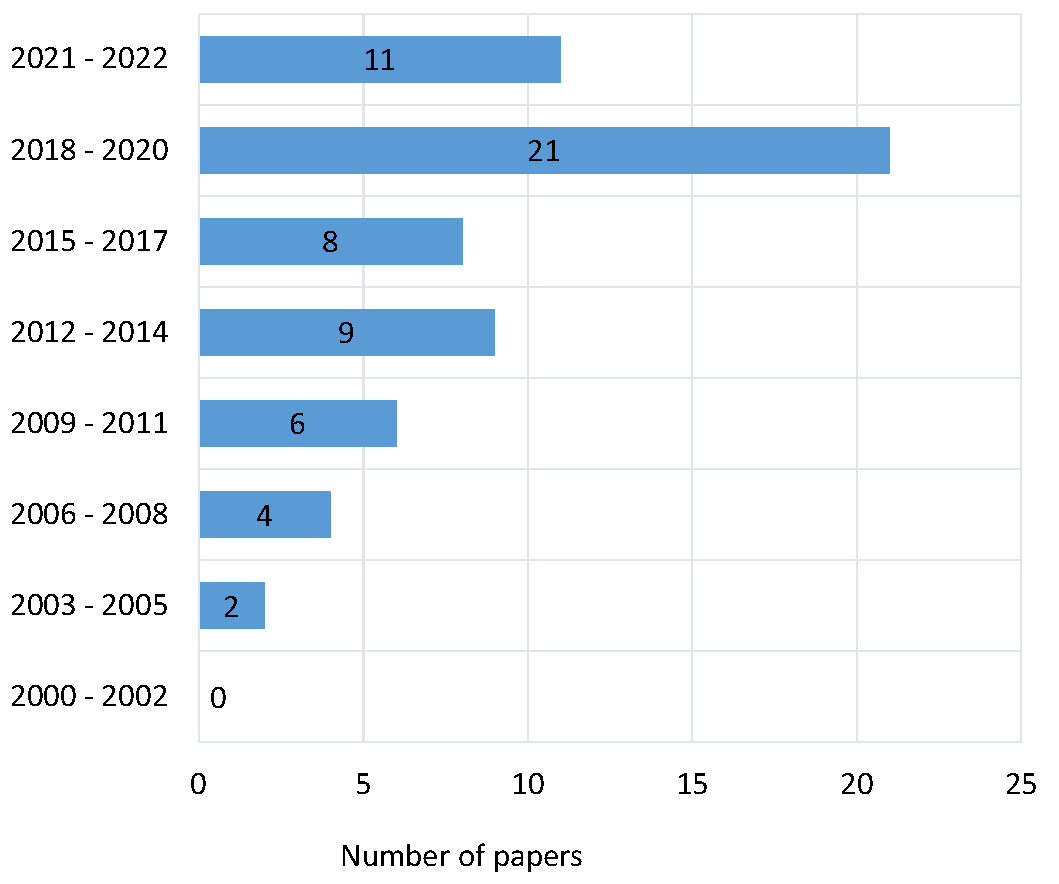
\includegraphics[scale = 0.5]{Chapters/Chapter2/Figures2/year1.pdf}
    \caption{Graph of Publication Year}
    \label{fig:litreview2-year}
\end{figure}

\subsubsection{Medical Context}
This subsection examines the articles' medical background, which can be grouped into two categories: the patients' condition area and the treatment's medical environment. Recall the definition of medical setting, which refers to the site where care is being provided, and condition area, which refers to whether the patient's medical condition was long- or short-term. 

To understand where these individuals were receiving care, three medical settings were examined. These are listed below:

\begin{itemize}
    \item Single Hospital
    \item Multiple Hospitals
    \item Community Care
\end{itemize}

Figure \ref{fig:litreview2-care} displays the results for the number of publications within each care setting. Single hospital settings were the most common with 33 papers (55\%). These papers concentrated on hospital wards, such as cardiac wards \cite{Cacciatore2012}, emergency departments (EDs) \cite{Bahrmann2018} and geriatric wards \cite{Tal2021}. Only thre papers, \cite{Hoben2019, Johnson2011, Welberry}, were based in the community. Hoben et al. \cite{Hoben2019} and Welberry et al. \cite{Welberry} evaluated the length of stay in nursing homes based on several factors, such as prior home care and policy variations. Johnson et al. \cite{Johnson2011} discussed the differences in location before being admitted to hospices and the effect this has on LOS. 

Interestingly, there were only two papers which explored hospital and community care settings simultaneously. Fan et al. \cite{Fan2021} used frailty as a predictor to determine the usage of healthcare, including LOS inside hospitals. Walsh et al. \cite{Walsh2020} analysed whether formal home care decreased LOS in hospitals. This suggests a possible direction for further study: using prediction models to calculate LOS across various services.

\begin{figure}[h!]
    \centering
    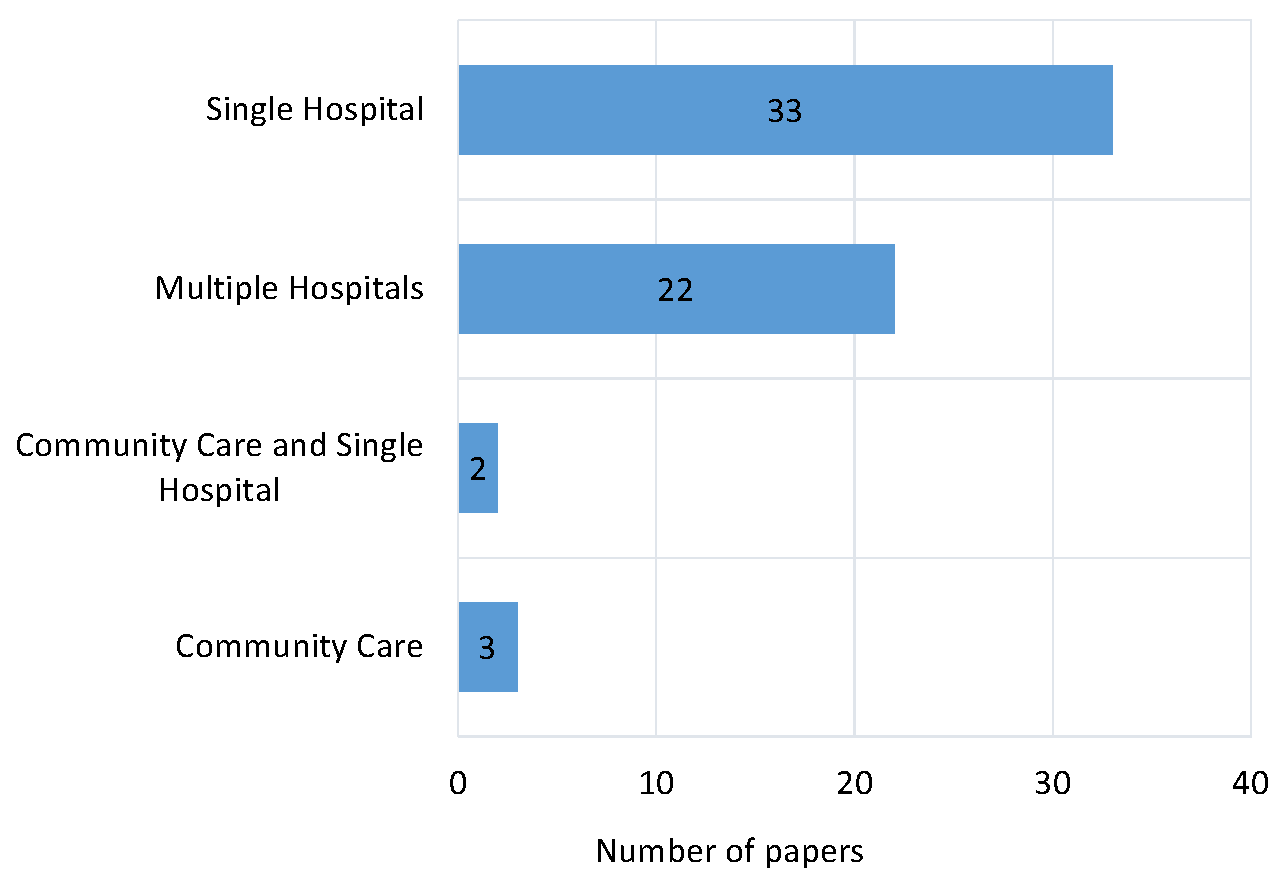
\includegraphics[scale=0.5]{Chapters/Chapter2/Figures2/care1.pdf}
    \caption{Number of publications within each care setting}
    \label{fig:litreview2-care}
\end{figure}

Another aspect to investigate is the condition area of a patient. There are three types of conditions included in this group: acute, chronic, and surgical. There are studies based on surgery in addition to the literature review covered in Section \ref{sec:litreview1}. Surgery papers are characterised as, medical disorders for which particular surgical procedures are used.

Figure \ref{fig:litreview2-condition} displays the quantity of papers in each medical condition category.

\begin{figure}[h!]
    \centering
    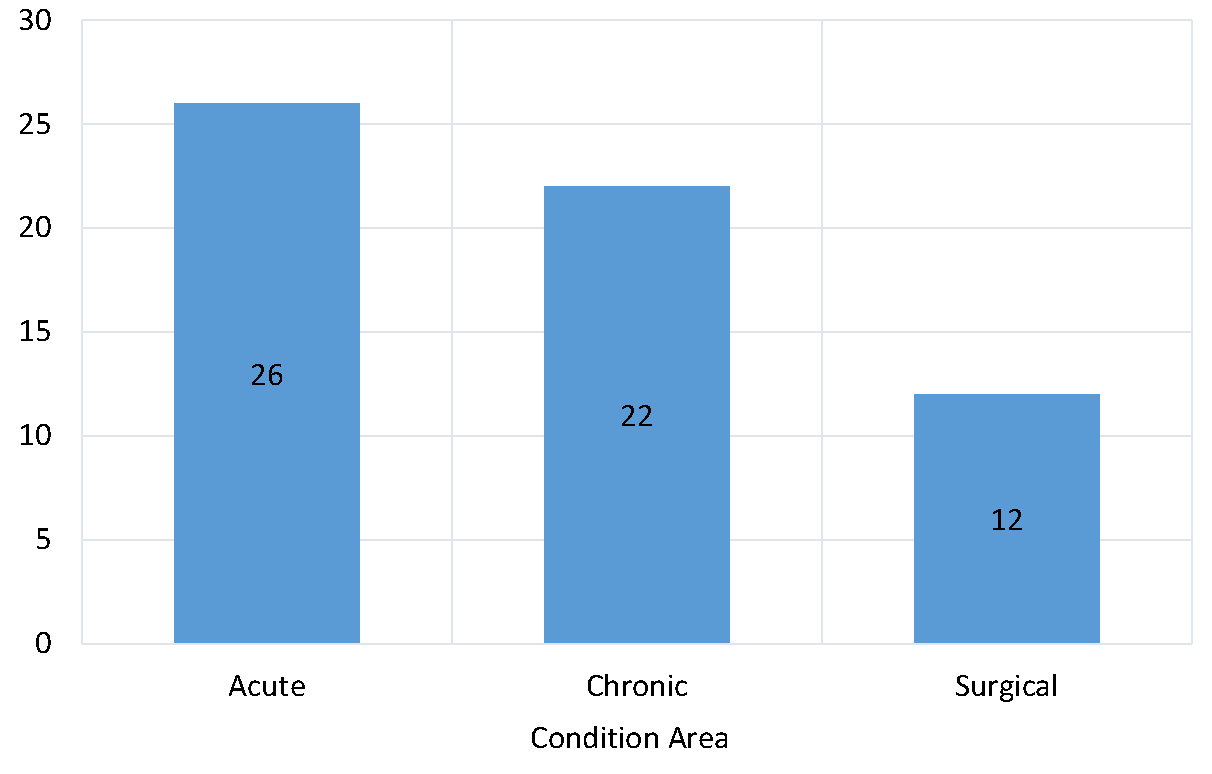
\includegraphics[scale=0.5]{Chapters/Chapter2/Figures2/area1.pdf}
    \caption{Condition categories of publications}
    \label{fig:litreview2-condition}
\end{figure}


ED's \cite{Bahrmann2018}, strokes \cite{Sommerfeld2011}, hip fractures \cite{Rajamaki2020}, and other acute medical conditions were present in the majority of papers (42\%). If these conditions are not treated, they can frequently lead to more serious medical problems. Only one of the 26 acute papers, Kim et al. \cite{Kim2018} was located across multiple hospitals; the other 25 were all based on single hospital wards. This shows that instead of overlapping with other hospitals or home care, acute facilities prefer to concentrate on their own setting. It is unexpected that there were more acute conditions than chronic ones considering that elderly and frail individuals have more chronic illnesses than the population of adults aged 16 to 64. Finally, there were twelve surgical articles focusing on various sub-specialities of surgery were included: Abdominal \cite{Marano2022}, cancer \cite{Raab2022}, cardiac \cite{Cacciatore2012,Kirfel2021,Pustavoitau2016}, colorectal \cite{AgasiIdenburg2019} and hip \cite{Justo2011,Willems2012}. In four of the publications \cite{Harvey2020,Jones2021, Zattoni2018, Zhao2020}, the surgical specialty was not specifically addressed.

\subsubsection{Methodological Content}
This subsection will analysis the technical aspect of the papers such as the goals of the research, the planning decision and the various LOS prediction techniques.

\subsubsubsection{Research Aims}
The papers can be categorised to define the direction of the research using the three main categories of research aim: examining, forecasting, and improving.

\begin{figure}[h!]
    \centering
    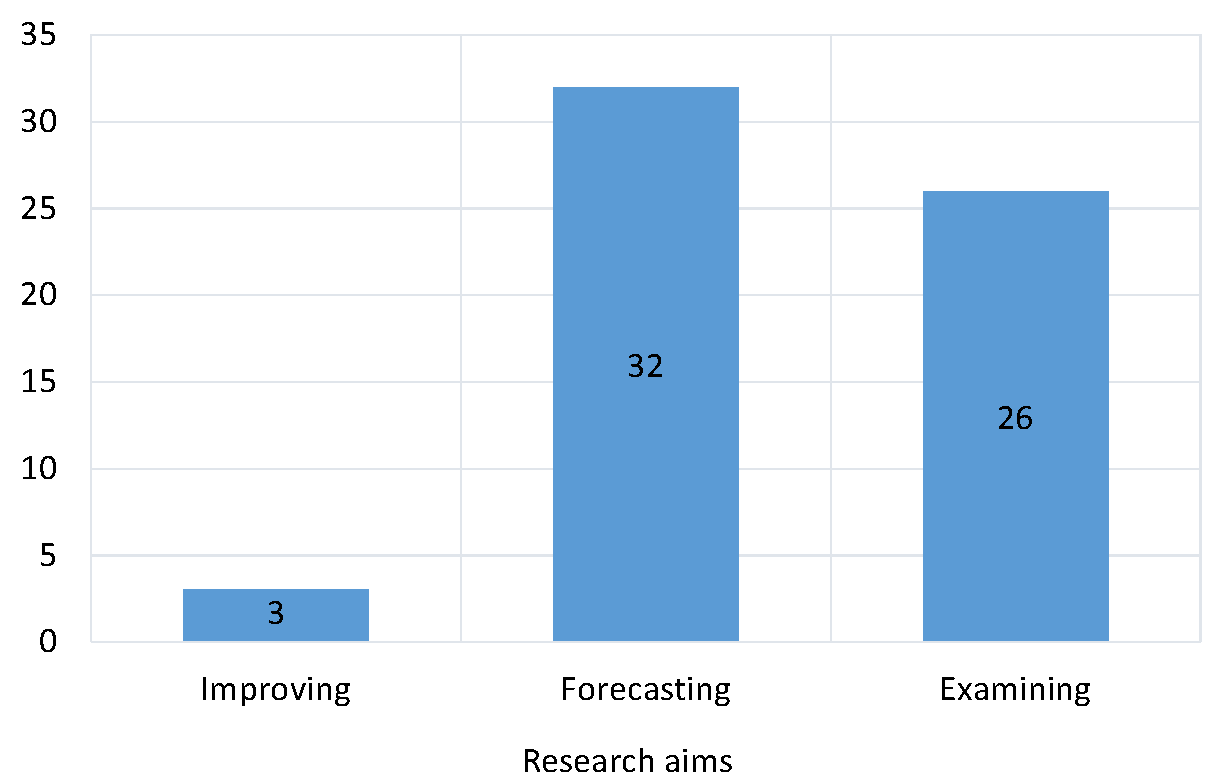
\includegraphics[scale=0.5]{Chapters/Chapter2/Figures2/aim1.pdf}
    \caption{Research aims of the papers}
    \label{fig:litreview2-aims}
\end{figure}

Figure \ref{fig:litreview2-aims} displays the quantity of papers in each of the research aim categories. Abe et al. \cite{Abe} using both examining and forecasting research aims by determining the effects of reducing polypharmacy on LOS on gastrointestinal surgery patients. 

    The findings indicate that, with 47\% of publications, forecasting is the most prevalent study goal. In these 32 studies, 15 were only concerned with LOS prediction \cite{Abe,Alyahya2017,Beauchet2018,Cacciatore2012,Hoben2019,Launay2018,Lisk2018,Marano2022,Marshall1,Nishino2019,Pustavoitau2016,Sommerfeld2011,Supervia2008,Takahashi2011,Willems2012}. The remaining 17 articles predicted other variables in addition to LOS such as, cost \cite{Feuerstadt2022,Tropea2016}, healthcare utilisation \cite{Fan2021}, mortality \cite{Bahrmann2018,Feuerstadt2022, Volpato2014} and hospital readmission \cite{Bahrmann2018, Morandi2013, Rajamaki2020}.

Only three publications examined how to improve LOS \cite{Basic2015,Hamdani,Walsh2020}. According to Basic and Khoo \cite{Basic2015}, the discovery of novel medical diagnoses would have an impact on funding models based on diagnosis-related groups (DRGs), but it might also improve patient care and their associated LOS. Hamdani et al. \cite{Hamdani} examined the use of Markov chains to model a hospital and the flow of elderly patients. Their model is then used to assess the effectiveness of intra-hospital care and predicting LOS.

\subsubsubsection{Planning Decisions}
Within Hulshof et al's. \cite{PHulshof} research on the taxonomic classification in healthcare systems, three different decision levels were discussed: strategic, tactical and operational.

Figure \ref{fig:lr2decisions} displays the number of publications by planning decision level. 

\begin{figure}[h!]
    \centering
    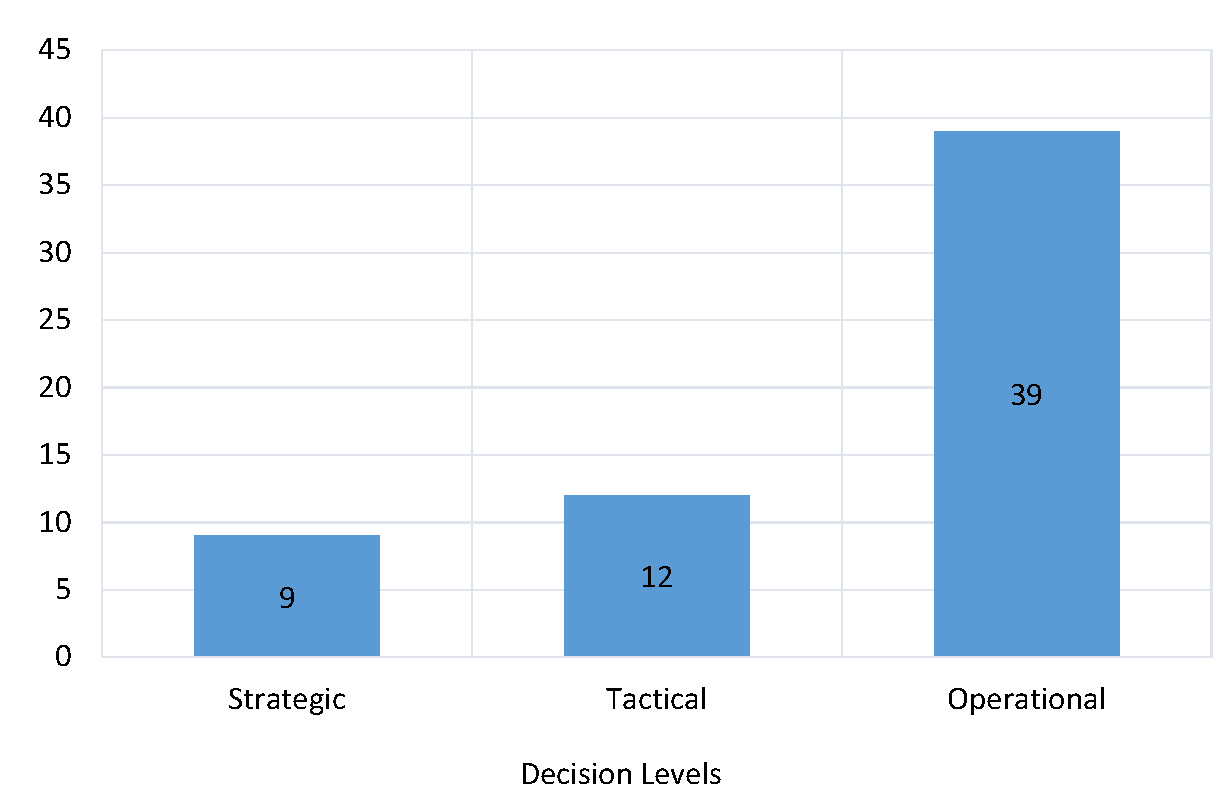
\includegraphics[scale=0.55]{Chapters/Chapter2/Figures2/decision1.pdf}
    \caption{Planning decision}
    \label{fig:lr2decisions}
\end{figure}

The majority of papers focused on operational planning, the day-to-day running of units. This is primarily due to the fact that the publications' main study goals involve predicting a patient's length of stay in the hospital, and the authors do not elaborate on this information to aid with long-term planning. 

There were only nine articles that made long-term planning decisions (strategic planning). This suggests that prediction modelling is more suited to short-term, day-to-day decisions rather than long-term, wider policy decisions. The research by Hoben et al. \cite{Hoben2019} is an illustration of a strategically categorised paper. The authors focused on LOS in nursing homes across three distinct Canadian regions. They investigated how LOS varied based on various regional policies as well as different characteristics of patients.

Figure \ref{fig:lr2cross1} displays the cross analysis between the planning decision and the medical setting. Despite having the fewest number of papers, strategic planning was the only planning decision to be addressed across all medical settings. Additionally, only a strategic level of consideration was given to community care settings. Operational planning was divided into papers based on single hospitals (59\%) and papers based in multiple hospitals (41\%). These findings demonstrate the applicability of prediction modelling in a variety of care settings, including short- and long-term care planning.

\begin{figure}[h!]
    \centering
    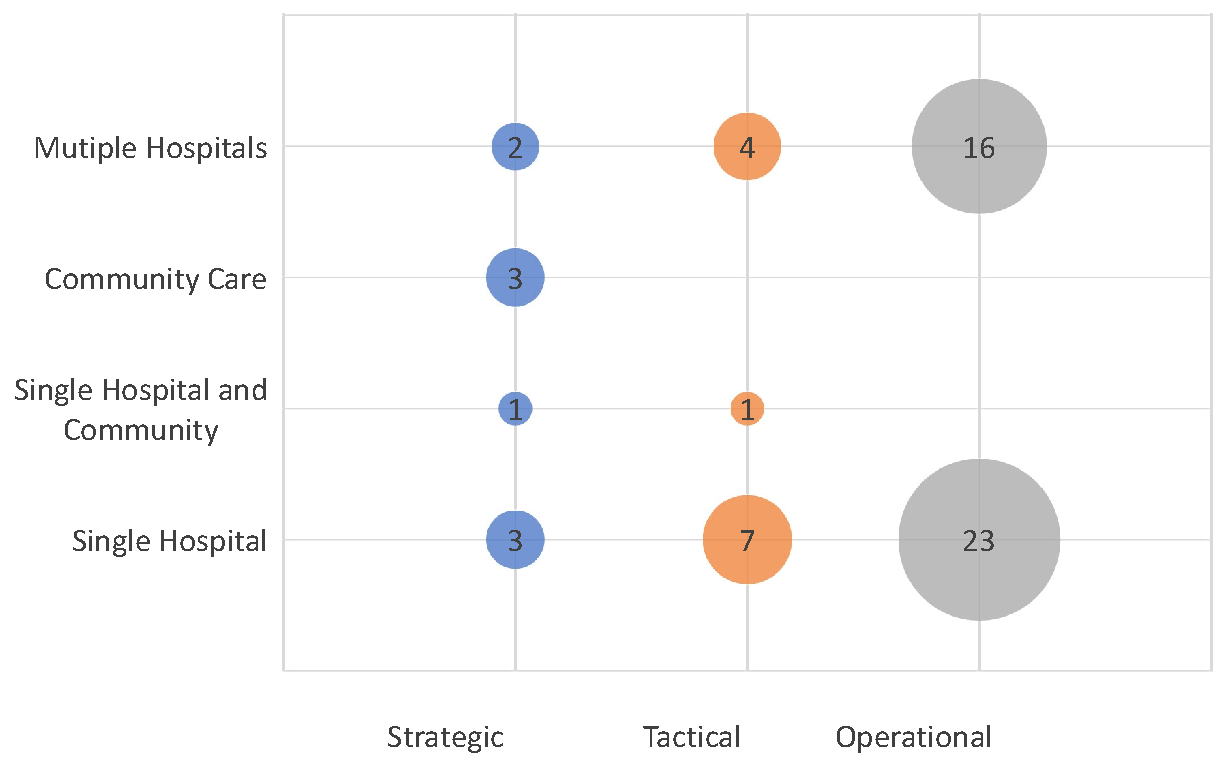
\includegraphics[scale=0.6]{Chapters/Chapter2/Figures2/decmed1.pdf}
    \caption{Cross analysis of planning decision and medical setting}
    \label{fig:lr2cross1}
\end{figure}

\subsubsubsection{Prediction Methods}
The final area to investigate was the prediction methods that have been utilised. 

Figure \ref{fig:lr2method} displays the quantity of each of the OR/MS methods.

\begin{figure}[h!]
    \centering
    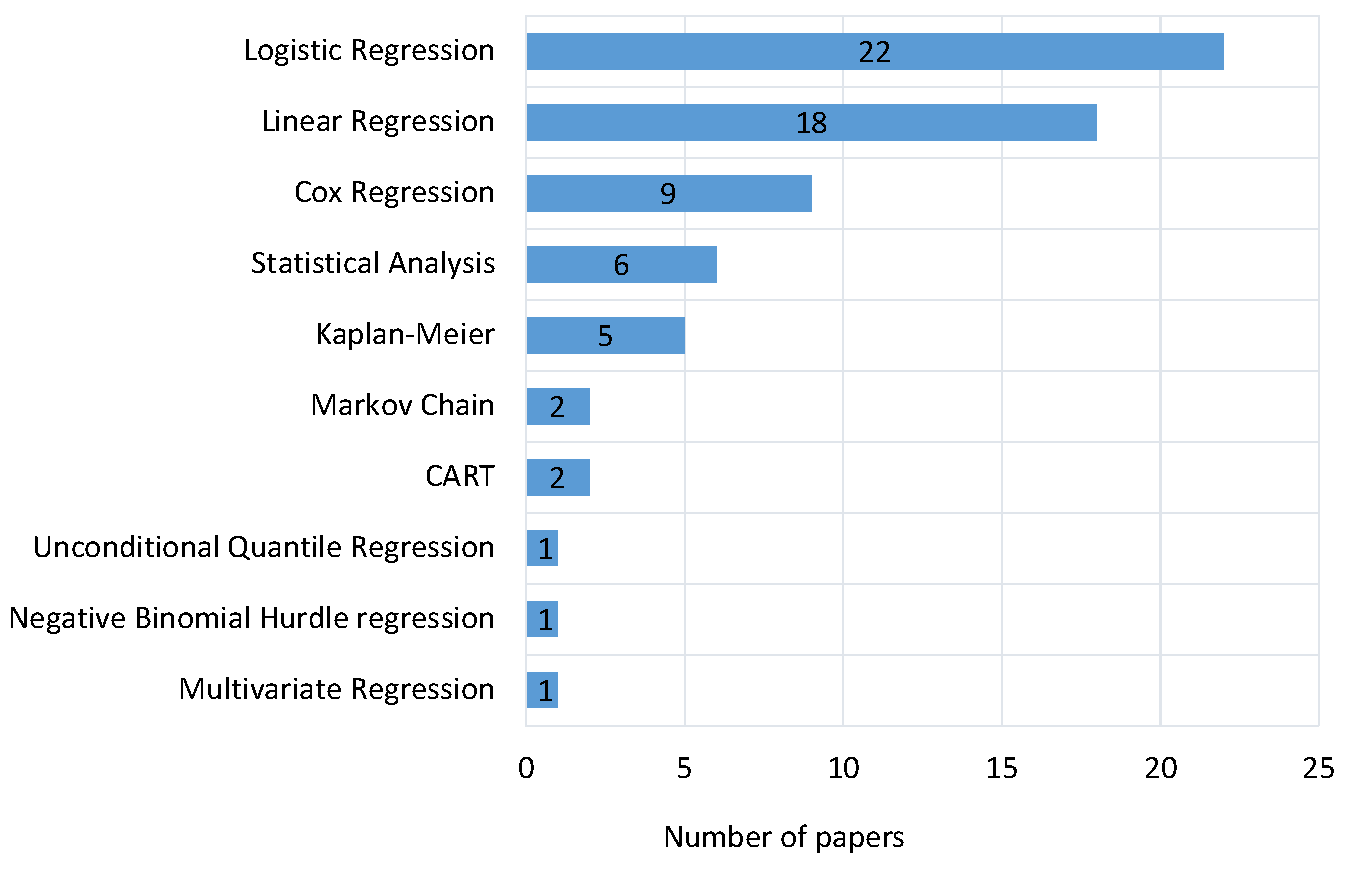
\includegraphics[scale=0.55]{Chapters/Chapter2/Figures2/method1.pdf}
    \caption{Quantity of publications by mathematical method}
    \label{fig:lr2method}
\end{figure}

Linear and Logistic regressions were the most prevalent techniques with 18 and 21 studies, respectively. Four articles, \cite{Adamis2017,Lisk2018,Motohashi2013,Naouri2022}, used both linear and logistic regression models in their research. Only two publications employed traditional hierarchical OR methods such as decision trees and CART \cite{Alyahya2017,Nishino2019}. In order to ascertain whether there was a relationship between LOS and preventable readmissions, Alyahya et al. \cite{Alyahya2017} developed decision trees. The authors discovered a direct correlation. Within the field of internal medicine, the authors were able to advise clinical decision makers on the recommended length of hospitalisation for patients. Nishino et al'.s \cite{Nishino2019} research involved building CART models to forecast long LOS's. Systolic blood pressure (155 mmHg) and serum albumin (3.4 g/dL, a blood protein present in albumin) readings were identified as lower bounds in to predicting long LOS's. 

There were three papers that used regression techniques that did not involve Cox, linear or logistic regression models. Multivariate multilevel regression was utilised by Chung et al. \cite{Chung2010} to identify the variables that affected patients' LOS in psychiatric wards. The type of medical institution, patient diagnosis, type of health insurance provider, and patient makeup of medical institutions were all shown to be significant determinants by the authors. Negative binomial hurdle regression models were used by Motzek et al. \cite{Motzek2018} to establish that longer hospital stays in Germany were caused by greater hospitalisation rates for dementia patients. Using unconditional quantile regression, Walsh et al. \cite{Walsh2020} identified a relationship between hospital LOS and formal home care.

Beauchet et al. \cite{Beauchet2018} utilised three methods within their research: cox and logistic regression with Kaplan-Meier models. The impact of several characteristics, such as a history of falls and temporal disorientation, on long hospital LOS's was examined by the authors.

Table \ref{tab:lr2methodsetting} refers to each papers' prediction method against its corresponding care setting. Since seven papers make use of various approaches, there are a total of 67 papers. Amongst the methods where there are five or greater papers published, a range of different care settings are used for the research. This demonstrates that, regardless of the situation, numerous strategies can be used in LOS modelling for elderly and frail patients. CART models are only used within single hospitals, and provides potential for research to focus on other care settings when using CART. Seven different methodologies were used in both single and multiple hospital settings, therefore having the most variety of approaches.

\begin{landscape}
    \begin{table}
        \centering\scalebox{0.63}{
        \begin{tabular}{ccccc|c}\toprule
            &\textbf{Single Hospital} & \textbf{Single Hospital and Community} & \textbf{Community Care} & \textbf{Multiple Hospitals} & \textbf{Total}  \\\midrule
            Logistic Regression & \cite{Abe,Adamis2017,Beauchet2018,Jones2021,Launay2018,Shen2019,Tropea2016,Zattoni2018,Zhao2020} &\cite{Fan2021}&\cite{Johnson2011}&\cite{AgasiIdenburg2019,Harvey2020,Hubbard2017,Lang2009,Lisk2018,Motohashi2013,Naouri2022,Rajamaki2020,Rubens2022,Shebeshi2021,Takahashi2011}& 22 \\
            Linear Regression &\cite{Adamis2017,Beauchet2013,Cacciatore2012,Chua2007,Justo2011,Kirfel2021,Pustavoitau2016,Raab2022,Snowden2004,Supervia2008,Willems2012} &&&\cite{Hasebe2018,Kim2018,Liotta2012,Lisk2018,Motohashi2013,Naouri2022,Wong2008}& 18\\
            Cox Regression & \cite{Basic2015,Beauchet2018,Hartley2019,Sommerfeld2011}&&\cite{Hoben2019,Welberry}&\cite{Kidd2014,Pilotto2016,Volpato2014}&9 \\
            Statistical Analysis& \cite{Beauchet2021,Harari2007,Marano2022,Tal2021,Wright2013} &&&\cite{Chen2020}&6 \\
            Kaplan-Meier & \cite{Bahrmann2018,Beauchet2018,Morandi2013}&&\cite{Johnson2011}&\cite{Feuerstadt2022}& 5 \\
            Markov Chain &\cite{Hamdani,Marshall1} &&&&2 \\
            CART & \cite{Alyahya2017,Nishino2019} &&&& 2\\
            Unconditional Quantile Regression & &\cite{Walsh2020}&&&1 \\
            Negative Binomial Hurdle Regression & &&&\cite{Motzek2018}& 1\\
            Multivariate Regression & &&&\cite{Chung2010}& 1\\\midrule
            \textbf{Total} & 36 & 2 & 4 & 25 & 67 \\\bottomrule 
            
        \end{tabular}}
        \caption{Setting and prediction method used within the published research}
        \label{tab:lr2methodsetting}
        \caption*{Note:Adamis et al. \cite{Adamis2017}, Beauchet et al. \cite{Beauchet2018}, 
 Johnson et al. \cite{Johnson2011}, Lisk et al. \cite{Lisk2018}, Motohashi et al. \cite{Motohashi2013}, Naouri et al. \cite{Naouri2022}, all utilise multiple methods and therefore appear multiple times within the table. This results in a total of 67.}
    \end{table}
\end{landscape}

\subsection{Common Themes}
Section \ref{sec:lr2results} provided an overview of prediction modelling for frail and elderly patients LOS in both hospitals and community care. Logistic regression was the most widely utilised method, with 22 papers developing these types of models. The last five years have seen the publication of more sophisticated techniques like CART, which are frequently derived from logistic and linear regression models. Operational planning was the most popular form of planning, indicating that prediction modelling is simpler to implement for daily operations of units and patient care. The papers include a variety of research objectives, with forecasting approaches being the most prevalent and frequently used to forecast patients' LOS. Finally,  hospitals have served as the primary environment for these publications, either based in a single hospital ward or analysed across multiple hospitals. The research identified through the Scopus search has demonstrated that a wide variety of OR/MS techniques can be applied to the care of elderly and frail LOS prediction modelling. Section \ref{sec:lr2researchgaps} will discuss the areas for future research.

\subsection{Research Gaps}\label{sec:lr2researchgaps}
Within ageing prediction modelling, the 60 studies found in this study addressed a wide range of facilities, regions, and patient types. Three significant gaps still exist in the literature, which could be the subject of future study.

\subsubsection{Gaps in terms of Methodology}

The 60 publications used ten distinct techniques, with a significant emphasis on linear and logistic regression. This is perhaps because the data lends itself nicely to these prediction techniques. There were five other approaches that accounted for 10\% of the paper methods, which used alternative prediction methods, indicating the potential for further research into these less commonly used techniques. The topic of elderly and frail prediction modelling underutilised more sophisticated and complex techniques like CART. In comparison to linear and logistic regression, CART models provide a deeper understanding into the data. Neural networks and clustering produced no relevant results in spite of being included in the Scopus search string in Table \ref{tab:Searchterms2}. Future studies may choose to concentrate on these hierarchical techniques, such as CART, clustering, and neural networks.

Patients with long LOS's typically account for a high proportion of overall bed days \cite{Quinn2007}. There are no laws or regulations regarding patient LOS, and it should be determined by when the patient is clinically fit for discharge. Bed occupancy has consistently exceeded 91\% in Canada \cite{OECD2023}, 85\% in England \cite{BMA2023} and 66\% in the USA \cite{CDCP2017}. There were only nine papers which specifically addressed on predicting the longer LOS in hospitals \cite{Abe,Beauchet2013,Beauchet2018,Cacciatore2012,Chen2020,Kirfel2021,Lang2009,Launay2018,Motohashi2013}. With the exception of Chen et al. \cite{Chen2020}, who employed statistical analysis, these articles only used linear and logistic regression techniques. Since trends in bed occupancy rates are still rising, particularly since the Covid-19 outbreak, projecting lengthy hospital LOSs and enacting policies to shorten them may lead to a decrease in occupancy rates.


% \begin{itemize}
%     \item I want to introduce CART as a potential method
%     \item how the linear and logistic regression models could be further developed into CART?
% \end{itemize}


\subsubsection{Gaps on the Intersection between Research Aims and Decision Levels}

Both the long-term and day-to-day planning scenarios should be taken into account for effective care planning. Only 21 publications examined the strategic and tactical decision levels, compared to the 39 papers that concentrated on the operational decision level. Decision-makers do not take into account how to best plan for the future because they are primarily concerned with day-to-day planning. Future, increased needs would not be satisfied as a result of this. All three locations for care, as well as the overlap between hospital wards and community care, were taken into account when determining strategic planning levels. On some level, this does indicate that all care facilities are being taken into account and analysed for the long-term horizon of LOS prediction modelling for elderly and frail patients. Policy makers will be able to make educated decisions based on these research papers regarding how to adapt units to future clinical and demographic changes.


The objectives of the research were also evaluated and divided into three groups: examining (26 papers), forecasting (32 papers) and improving (3 papers). Eight of the ten different methods were used to achieve the most popular study goal, forecasting. With 17 publications, forecasting was primarily employed to predict numerous parameters as opposed to only LOS (15 papers). This demonstrates how LOS prediction can support care planning by working in conjunction with other predictors. Only three studies, all of which took place in a single hospital, were related to the improving research aim \cite{Hamdani,Basic2015,Walsh2020}. Although it does open up a new line of inquiry for researchers, it may also imply that the study methods these publications examined were simpler to apply to single settings.
 
% \begin{itemize}
%     \item CART
%     \item research aims and decision levels
%     \item interaction between medical settings
%     \item The majority of papers focused on operational planning, the day-to-day running of units. This is primarily due to the fact that the publications' main study goals involve predicting a patient's length of stay in the hospital, and the authors do not elaborate on this information to aid with long-term planning. 
% \end{itemize}

\subsubsection{Shortcomings on the Intersections between Medical Settings}

There were only five studies that addressed LOS prediction modelling in the context of community care \cite{Fan2021,Hoben2019,Johnson2011,Walsh2020,Welberry}. This shows that LOS prediction modelling may not be well adapted to community care settings, given that patients are often unlikely to return to their own homes after being admitted to a nursing or care facility. Fan et al's. \cite{Fan2021} and Walsh et al.'s \cite{Walsh2020} research using a single hospital and community care setting were the sole crossovers between community and hospital settings. This presents an opportunity to examine if patients who receive some form of community care have different LOS's when admitted. Two potential hypotheses could be tested: whether patients are discharged sooner because they have a home to return to in the community and do not bed block, or because these patients are typically sicker and take longer to recover as they are already receiving care and hence stay in hospital for longer.

In total, 22 studies addressed multiple hospital settings. Although being able to forecast LOS at the time of admission can help with resource allocation for a patient's hospital stay, none of the publications were found to do more than merely investigate the variables that influence LOS. The development of these LOS prediction models and their use in resource planning would fill a significant research gap. 
Nine of the 22 multiple hospital papers, \cite{Hubbard2017,Kim2018,Liotta2012,Lisk2018,Naouri2022,Pilotto2016,Shebeshi2021,Volpato2014,Wong2008}, did not concentrate on a particular disease but instead analysed the elderly admission and were able to compare LOS based on various illnesses. These publications do not, however, examine or make forecasts for the future on a bigger scale. This leaves open the possibility for future studies to examine the effects of various medical conditions on patient demands and LOS, as well as how these factors may alter over time based on clinical and demographic changes.

% \begin{itemize}
%     \item where is there research available for multiple hospitals
%     \item what do examining and improving look at
%     \item want to make it so
%     \item use LOS prediction across hospitals to plan bed numbers based on these LOS
% \end{itemize}

\subsection{Literature Review Findings}\label{sec:lr2findings}

This section has established a framework for categorising general, medical, and methodological components of prediction modelling for frail and elderly patients. The literature on healthcare has been categorised for a total of 23 years. The significance of bridging the gap between GG journals and more conventional health mathematics journals (HPS, IE, and MI) has been emphasised, similar to the literature review in Section \ref{sec:litreview1}. As a consequence, the same three  overarching research opportunities, as Section \ref{sec:litreview1}, have been identified.

\begin{enumerate}
    \item The use of linear and logistic regression was the focus of 60\% of the publications.  Despite the fact that they were employed in conjunction with other techniques, this leaves potential for further study to build on other methods techniques such as CART. Given that our study only found six publications utilising this strategy, it might be further developed by integrating other strategies to produce a more diverse model. The kind of prediction method employed may vary depending on the environment and types of data that are regularly collected. Another avenue for investigation is the application of other hierarchical techniques, such as neural networks or clustering, which, despite being part of the Scopus search term, failed to yield any pertinent outcomes.

    \item Predicting LOS for elderly and frail patients across the care pathway would benefit from more research. Only two studies with a single hospital and community care as their primary settings were identified. Due to the bed blockage issue that many healthcare facilities are experiencing, it is crucial that hospitals and community care are integrated. When a patient is medically fit for release but cannot be transferred because there is nowhere for them to go, this is known as bed blocking. This frequently happens as a result of the time it takes to arrange for people who need home care or who need to be admitted to a nursing or care facility. As a result, this leads to longer LOS in hospitals and this cannot be resolved without adequate care in the community. This is supported by the discovery of just nine studies with a specific focus on predicting longer LOS's within hospitals. 

    \item The final research possibility focuses on the increased demands and pressures that healthcare facilities are currently experiencing. None of the publications addressed the possibility that hospital LOS would rise in response to rising demand for admissions of elderly and frail patients. First of all, if there is a greater influx of patients, staff would have to care for more patients and as a result become overworked, which might significantly affect patients' recovery times. Additionally, because there would be more demand for inpatient treatments like radiology or pathology, patients would have to wait longer for these examinations, extending their LOS.
    
\end{enumerate}


\section{Summary}\label{sec:litreviewsum}
The practice of OR/MS approaches in the planning of care for the frail and elderly was the main topic of this chapter's literature reviews. The underutilisation of OR/MS techniques, the absence of comprehensive holistic care planning, and the implications of increases in demand on healthcare systems have all been noted as gaps in the literature. Within this thesis, we seek to address all three aspects by using underutilised OR/MS methods and applying them to multiple hospitals in Chapter \ref{chp:Experimental Analysis} and discussing growing demand in Chapter \ref{chp:Discussion} using scenario analysis.

The application of OR/MS methods to elderly and frail patients literature review (Section \ref{sec:litreview1}) included a higher quantity of strategic level publications, hence the two literature reviews did dispute in terms of planning decisions. There was a stronger emphasis on operational planning choices in the literature review for  the hierarchical prediction models for patients' LOS literature review (Section \ref{sec:litreview2}). Therefore, all three planning decisions will be examined in this research, including how to plan the day-to-day running of units while also taking into consideration long-term demands and predictions for elderly and frail patients.

In the following chapter, Chapter \ref{chp:predictive}, we discuss a number of the predictive analytical methods identified within from the literature reviews. Through a realistic, simplified example illustrating the procedures and outcomes, the methods will be applied to the case of frail and elderly patients. 

\end{document}
